%%%%%%%%%%%%%%%%%%%%%%%%%%%%%%%%%%%%%%%%%
%DIF LATEXDIFF DIFFERENCE FILE
%DIF DEL manuscript-352b54a.tex   Wed Sep 19 21:06:57 2018
%DIF ADD manuscript-a12dad5.tex   Wed Sep 19 21:07:05 2018
% NIH Grant Proposal for the Specific Aims and Research Plan Sections
% LaTeX Template
% Version 1.0 (21/10/13)
%
% This template has been downloaded from:
% http://www.LaTeXTemplates.com
%
% Original author:
% Erick Tatro (erickttr@gmail.com) with modifications by:
% Vel (vel@latextemplates.com)
%
% Adapted from:
% J. Hrabe (http://www.magalien.com/public/nih_grants_in_latex.html)
%
% License:
% CC BY-NC-SA 3.0 (http://creativecommons.org/licenses/by-nc-sa/3.0/)
%
%%%%%%%%%%%%%%%%%%%%%%%%%%%%%%%%%%%%%%%%%

%----------------------------------------------------------------------------------------
%	PACKAGES AND OTHER DOCUMENT CONFIGURATIONS
%----------------------------------------------------------------------------------------
\PassOptionsToPackage{unicode=true}{hyperref} % options for packages loaded elsewhere
\PassOptionsToPackage{hyphens}{url}
\PassOptionsToPackage{dvipsnames,svgnames*,x11names*}{xcolor}
%
%% DRS packages to load based on NIH.
\documentclass[11pt,notitlepage]{article}

% \usepackage[T1]{fontenc}
\linespread{1.15} % A little extra line spread is better for the Palatino font
\usepackage{amsfonts, amsmath, amsthm, amssymb} % For math fonts, symbols and environments
\usepackage{graphicx} % Required for including images
\usepackage{booktabs} % Top and bottom rules for table
\usepackage{wrapfig} % Allows in-line images
\usepackage{setspace}
\usepackage[labelfont=bf,font=small]{caption} % Make figure numbering in captions bold
\captionsetup{belowskip=-4pt,aboveskip=4pt}
\usepackage[top=0.5in,bottom=0.5in,left=0.5in,right=0.5in,includeheadfoot]{geometry} % Reduce the size of the margin
\usepackage[utf8]{inputenc}
\usepackage[T1]{fontenc}
\usepackage[greek,english]{babel}
% For switching to xelatex if unicode detected...
 \usepackage[no-math]{fontspec}
 \setmainfont{Helvetica}
 %\usepackage{mathspec}
 %\setmathfont(Digits,Latin)[Uppercase=Italic,Lowercase=Italic]{Helvetica}
 %\setmathfont(Greek)[Uppercase=Regular,Lowercase=Regular]{Helvetica}
 
\usepackage{fancyhdr}
\renewcommand{\headrulewidth}{0pt}
\pagestyle{fancy}
%\setlength{\headheight}{15.2pt}


 \usepackage[small,compact]{titlesec}
 \titlespacing{\title}{-2in}{0ex}{-3in}
 \titlespacing{\section}{0pt}{\parskip}{-\parskip}
 \titlespacing{\subsection}{0pt}{-\parskip}{-\parskip}
 \titlespacing{\subsubsection}{0pt}{0pt}{-\parskip}
 \titleformat{\section}%
  [hang]% <shape>
  {\normalfont\bfseries}% <format>
  {}% <label>
  {0pt}% <sep>
  {}% <before code>

\renewcommand{\thesection}{}
\renewcommand{\thesubsection}{\arabic{subsection}}

\usepackage{amssymb,amsmath}
\usepackage{ifxetex,ifluatex}
\usepackage{fixltx2e} % provides \textsubscript
\ifnum 0\ifxetex 1\fi\ifluatex 1\fi=0 % if pdftex
  \usepackage[T1]{fontenc}
  \usepackage[utf8]{inputenc}
  \usepackage{textcomp} % provides euro and other symbols
\else % if luatex or xelatex
%%  \usepackage{unicode-math}
%  \defaultfontfeatures{Ligatures=TeX,Scale=MatchLowercase}
    \setmainfont[]{Helvetica}
    \setsansfont[]{Helvetica}
%\fi
% use upquote if available, for straight quotes in verbatim environments
\IfFileExists{upquote.sty}{\usepackage{upquote}}{}
% use microtype if available
\IfFileExists{microtype.sty}{%
\usepackage[]{microtype}
\UseMicrotypeSet[protrusion]{basicmath} % disable protrusion for tt fonts
}{}
\IfFileExists{parskip.sty}{%
\usepackage{parskip}
}{% else
\setlength{\parindent}{0pt}
\setlength{\parskip}{6pt plus 2pt minus 1pt}
}
\usepackage{xcolor}
\usepackage{hyperref}
\hypersetup{
            pdftitle={Membranes, motors, and molecular modeling},
            pdfauthor={David R. Slochower},
            colorlinks=true,
            linkcolor=Maroon,
            citecolor=Blue,
            urlcolor=Blue,
            breaklinks=true}
\urlstyle{same}  % don't use monospace font for urls
\usepackage{graphicx,grffile}
\makeatletter
\def\maxwidth{\ifdim\Gin@nat@width>\linewidth\linewidth\else\Gin@nat@width\fi}
\def\maxheight{\ifdim\Gin@nat@height>\textheight\textheight\else\Gin@nat@height\fi}
\makeatother
% Scale images if necessary, so that they will not overflow the page
% margins by default, and it is still possible to overwrite the defaults
% using explicit options in \includegraphics[width, height, ...]{}
\setkeys{Gin}{width=\maxwidth,height=\maxheight,keepaspectratio}
\setlength{\emergencystretch}{3em}  % prevent overfull lines
\providecommand{\tightlist}{%
  \setlength{\itemsep}{0pt}\setlength{\parskip}{0pt}}
\setcounter{secnumdepth}{5}
% Redefines (sub)paragraphs to behave more like sections
\ifx\paragraph\undefined\else
\let\oldparagraph\paragraph
\renewcommand{\paragraph}[1]{\oldparagraph{#1}\mbox{}}
\fi
\ifx\subparagraph\undefined\else
\let\oldsubparagraph\subparagraph
\renewcommand{\subparagraph}[1]{\oldsubparagraph{#1}\mbox{}}
\fi

% set default figure placement to htbp
\makeatletter
\def\fps@figure{htbp}
\makeatother


%DRS
\title{\large \vspace{-0.75in} \textbf{Membranes, motors, and molecular modeling} \vspace{-1in} }
\fancypagestyle{title}{%
  \setlength{\headheight}{22pt}%
  \fancyhf{}% No header/footer
  \renewcommand{\headrulewidth}{0pt}% No header rule
  \renewcommand{\footrulewidth}{0pt}% No footer rule
  \fancyfoot[C]{\thepage}% Page number in Centre of footer
  \fancyhead[L]{David R.~Slochower}
  \fancyhead[R]{Research Plan}
}%
 \lhead{David R.~Slochower}
 \rhead{Research Plan}

% \pagestyle{empty} % Remove page numbers

\date{}
%DIF PREAMBLE EXTENSION ADDED BY LATEXDIFF
%DIF UNDERLINE PREAMBLE %DIF PREAMBLE
\RequirePackage[normalem]{ulem} %DIF PREAMBLE
\RequirePackage{color}\definecolor{RED}{rgb}{1,0,0}\definecolor{BLUE}{rgb}{0,0,1} %DIF PREAMBLE
\providecommand{\DIFaddtex}[1]{{\protect\color{blue}\uwave{#1}}} %DIF PREAMBLE
\providecommand{\DIFdeltex}[1]{{\protect\color{red}\sout{#1}}}                      %DIF PREAMBLE
%DIF SAFE PREAMBLE %DIF PREAMBLE
\providecommand{\DIFaddbegin}{} %DIF PREAMBLE
\providecommand{\DIFaddend}{} %DIF PREAMBLE
\providecommand{\DIFdelbegin}{} %DIF PREAMBLE
\providecommand{\DIFdelend}{} %DIF PREAMBLE
%DIF FLOATSAFE PREAMBLE %DIF PREAMBLE
\providecommand{\DIFaddFL}[1]{\DIFadd{#1}} %DIF PREAMBLE
\providecommand{\DIFdelFL}[1]{\DIFdel{#1}} %DIF PREAMBLE
\providecommand{\DIFaddbeginFL}{} %DIF PREAMBLE
\providecommand{\DIFaddendFL}{} %DIF PREAMBLE
\providecommand{\DIFdelbeginFL}{} %DIF PREAMBLE
\providecommand{\DIFdelendFL}{} %DIF PREAMBLE
%DIF HYPERREF PREAMBLE %DIF PREAMBLE
\providecommand{\DIFadd}[1]{\texorpdfstring{\DIFaddtex{#1}}{#1}} %DIF PREAMBLE
\providecommand{\DIFdel}[1]{\texorpdfstring{\DIFdeltex{#1}}{}} %DIF PREAMBLE
\newcommand{\DIFscaledelfig}{0.5}
%DIF HIGHLIGHTGRAPHICS PREAMBLE %DIF PREAMBLE
\RequirePackage{settobox} %DIF PREAMBLE
\RequirePackage{letltxmacro} %DIF PREAMBLE
\newsavebox{\DIFdelgraphicsbox} %DIF PREAMBLE
\newlength{\DIFdelgraphicswidth} %DIF PREAMBLE
\newlength{\DIFdelgraphicsheight} %DIF PREAMBLE
% store original definition of \includegraphics %DIF PREAMBLE
\LetLtxMacro{\DIFOincludegraphics}{\includegraphics} %DIF PREAMBLE
\newcommand{\DIFaddincludegraphics}[2][]{{\color{blue}\fbox{\DIFOincludegraphics[#1]{#2}}}} %DIF PREAMBLE
\newcommand{\DIFdelincludegraphics}[2][]{% %DIF PREAMBLE
\sbox{\DIFdelgraphicsbox}{\DIFOincludegraphics[#1]{#2}}% %DIF PREAMBLE
\settoboxwidth{\DIFdelgraphicswidth}{\DIFdelgraphicsbox} %DIF PREAMBLE
\settoboxtotalheight{\DIFdelgraphicsheight}{\DIFdelgraphicsbox} %DIF PREAMBLE
\scalebox{\DIFscaledelfig}{% %DIF PREAMBLE
\parbox[b]{\DIFdelgraphicswidth}{\usebox{\DIFdelgraphicsbox}\\[-\baselineskip] \rule{\DIFdelgraphicswidth}{0em}}\llap{\resizebox{\DIFdelgraphicswidth}{\DIFdelgraphicsheight}{% %DIF PREAMBLE
\setlength{\unitlength}{\DIFdelgraphicswidth}% %DIF PREAMBLE
\begin{picture}(1,1)% %DIF PREAMBLE
\thicklines\linethickness{2pt} %DIF PREAMBLE
{\color[rgb]{1,0,0}\put(0,0){\framebox(1,1){}}}% %DIF PREAMBLE
{\color[rgb]{1,0,0}\put(0,0){\line( 1,1){1}}}% %DIF PREAMBLE
{\color[rgb]{1,0,0}\put(0,1){\line(1,-1){1}}}% %DIF PREAMBLE
\end{picture}% %DIF PREAMBLE
}\hspace*{3pt}}} %DIF PREAMBLE
} %DIF PREAMBLE
\LetLtxMacro{\DIFOaddbegin}{\DIFaddbegin} %DIF PREAMBLE
\LetLtxMacro{\DIFOaddend}{\DIFaddend} %DIF PREAMBLE
\LetLtxMacro{\DIFOdelbegin}{\DIFdelbegin} %DIF PREAMBLE
\LetLtxMacro{\DIFOdelend}{\DIFdelend} %DIF PREAMBLE
\DeclareRobustCommand{\DIFaddbegin}{\DIFOaddbegin \let\includegraphics\DIFaddincludegraphics} %DIF PREAMBLE
\DeclareRobustCommand{\DIFaddend}{\DIFOaddend \let\includegraphics\DIFOincludegraphics} %DIF PREAMBLE
\DeclareRobustCommand{\DIFdelbegin}{\DIFOdelbegin \let\includegraphics\DIFdelincludegraphics} %DIF PREAMBLE
\DeclareRobustCommand{\DIFdelend}{\DIFOaddend \let\includegraphics\DIFOincludegraphics} %DIF PREAMBLE
\LetLtxMacro{\DIFOaddbeginFL}{\DIFaddbeginFL} %DIF PREAMBLE
\LetLtxMacro{\DIFOaddendFL}{\DIFaddendFL} %DIF PREAMBLE
\LetLtxMacro{\DIFOdelbeginFL}{\DIFdelbeginFL} %DIF PREAMBLE
\LetLtxMacro{\DIFOdelendFL}{\DIFdelendFL} %DIF PREAMBLE
\DeclareRobustCommand{\DIFaddbeginFL}{\DIFOaddbeginFL \let\includegraphics\DIFaddincludegraphics} %DIF PREAMBLE
\DeclareRobustCommand{\DIFaddendFL}{\DIFOaddendFL \let\includegraphics\DIFOincludegraphics} %DIF PREAMBLE
\DeclareRobustCommand{\DIFdelbeginFL}{\DIFOdelbeginFL \let\includegraphics\DIFdelincludegraphics} %DIF PREAMBLE
\DeclareRobustCommand{\DIFdelendFL}{\DIFOaddendFL \let\includegraphics\DIFOincludegraphics} %DIF PREAMBLE
%DIF END PREAMBLE EXTENSION ADDED BY LATEXDIFF

\begin{document}
% DRS
\lhead{David R.~Slochower}

\maketitle
%DRS
\thispagestyle{title}


My research interests center on uncovering the physical principles that
underlie biological and chemical phenomena. I try to create more
accurate molecular simulations by improving physics-based force fields
and combining new simulation procedures with nonequilibrium analytical
tools. I will extend my previous work on biological membranes to
elucidate driving forces behind the formation of membrane domains
featuring phosphoinositides. I will also run simulations of synthetic
molecular motors, such as those designed by Ben Feringa, to characterize
their mechanical properties. Finally, I will participate in a systematic
overhaul of force field science, changing the way force fields are built
and how they are distributed, by focusing on transparent and rigorous
optimization criteria, in an open setting. These investigations will
provide a detailed accounting of the physical principles that are at
work in biological systems. My undergraduate degree in physics combined
with my graduate work in biochemistry and biophysics, together with my
postdoctoral training in computational chemistry, makes me well suited
to this research plan. Each aim of my detailed research plan focuses on
a physical or chemical question at the heart of molecular motion.

\DIFaddbegin \DIFadd{The interface between physics and biology is an active, growing area of
science with many unanswered questions. My research program will
investigate the physical principles that underlie biological and
chemical phenomena, providing new insight into the complex behavior of
cell membranes, the operation of molecular motors, and more rigorous
methods of developing force fields. In particular, I will focus on three
areas that bridge theory, modeling, and simulations: (1) the formation
of ion-mediated phospholipid domains, (2) the out-of-equilibrium
statistical mechanics of synthetic rotary motors, and (3) open source
development of new force fields for drug design incorporating binding
thermodynamics.
}

\DIFadd{Method development is vital to my research interests because it allows
theory and simulation to gain new perspectives on challenging problems.
I will extend my previous work on biological membranes to elucidate the
driving forces behind clusters featuring phosphoinositides. I will use
nonequilibrium kinetic modeling to suggest new design principles for
molecular motors. Finally, I will participate in a systematic overhaul
of force field science, changing the way force fields are built and how
they are distributed, by focusing on transparent and rigorous
optimization criteria, in an open setting.
}

\DIFadd{\textcolor{blue}{\textbf{Insert university-specific paragraph here.}}
}

\DIFaddend \hypertarget{summary-of-previous-research}{%
\section{Summary of previous
research}\label{summary-of-previous-research}}

\hypertarget{improving-free-energy-calculations}{%
\subsection{Improving free energy
calculations}\label{improving-free-energy-calculations}}

Accurate binding thermodynamics calculations remain one of the central
goals of biomolecular simulations. While in the Gilson group, I
contributed to an overall evaluation of more than ten different methods,
from research groups around the world, used to compute host-guest
binding free energies and
enthalpies\textsuperscript{\protect\hyperlink{ref-BGsUYQln}{1}}. As part
of that work, I extended our own method
(attach-pull-release\textsuperscript{\protect\hyperlink{ref-uzHaEv9Z}{2}})
by completely rewriting the code in Python and adding several advanced
features enabling larger and more challenging systems to be used (this
code is available on
\href{https://www.github.com/slochower/pAPRika}{GitHub}). More recently,
I have also worked on assessing the efficiency and reproducibility of
how different algorithms converge toward free energy estimates
(forthcoming publication).

\hypertarget{the-evolution-of-molecular-motors}{%
\subsection{The evolution of molecular
motors}\label{the-evolution-of-molecular-motors}}

Biological motors are enzymes that use chemical energy to drive
directional motion. Although motor proteins must have arisen through
random mutation and natural selection, it is not clear how the
evolutionary leap from non-motor enzymes to molecular motors could have
occurred. I showed that any chiral molecule driven out of equilibrium
should undergo cycles of conformational
change\textsuperscript{\protect\hyperlink{ref-1BfYw0gk2}{3}}. This work
was highlighted by
\href{http://ucsdhealthsciences.tumblr.com/post/173707350285/its-not-intelligent-design-so-how-did}{UCSD}
and
\href{https://www.cell.com/biophysj/fulltext/S0006-3495(18)30444-2}{``New
and Notable''} in Biophysical Journal.

\hypertarget{the-design-of-new-force-fields}{%
\subsection{The design of new force
fields}\label{the-design-of-new-force-fields}}

As part of the open force field consortium---a collaboration with
Dr.~David Mobley, Dr.~John Chodera, Dr.~Michael Shirts, Dr.~Lee-Ping
Wang, and Dr.~Chris Bayly--- I participated in the effort to build new
molecular mechanics force fields based on direct chemical perception
instead of indirect, atom-type based approaches (forthcoming
publication). I have also contributed to the design, coding, and
implementation of a new force field format---SMIRKS Native Open Force
Field (SMIRNOFF)---based on a hierarchical structure that supports
customized combining rules, partial bond orders, polarizability, and
other advanced features. The tools and data are open source and
available on \href{https://github.com/openforcefield}{GitHub}.

\hypertarget{simulations-of-complex-membranes}{%
\subsection{Simulations of complex
membranes}\label{simulations-of-complex-membranes}}

Continuing the work that I started during graduate school at the
University of
Pennsylvania\textsuperscript{\protect\hyperlink{ref-1G0A01ZNq}{4}--\protect\hyperlink{ref-1AHXI1BtY}{8}},
I'm interested in simulating increasingly complex, and thus more
physiologically relevant, models of biological membranes. We recently
reported (forthcoming publication) how the interplay between lipid
species, cholesterol, counterions, and water near the membrane interface
can lead to the formation of nano-scale lipid clusters. A natural next
step is to understand the role proteins play in stabilizing these
clusters, as discussed below.

\hypertarget{detailed-research-plan}{%
\section{Detailed research plan}\label{detailed-research-plan}}

\hypertarget{how-are-highly-enriched-clusters-of-negatively-charged-phospholipids-stabilized}{%
\subsection{How are highly enriched clusters of negatively charged
phospholipids
stabilized?}\label{how-are-highly-enriched-clusters-of-negatively-charged-phospholipids-stabilized}}

Phosphoinositides are a minor class of lipids located on the inner
leaflet of the plasma membrane, found at about 0.5 mole percent of all
phospholipids in mammalian cells (10-100 μM), that have an outsized
biological role. This class of lipids participates in myriad cell
processes including attachment of the cytoskeleton, membrane fusion,
vesiculation, and both activation and inhibition of
enzymes\textsuperscript{\protect\hyperlink{ref-GGlssBvj}{9}}. Disruption
in signaling pathways associated with the phosphoinositides have been
implicated in several cancers as well as Charcot-Marie-Tooth disease
along with other neurodegenerative
disorders\textsuperscript{\protect\hyperlink{ref-8Xw2kuUO}{10}--\protect\hyperlink{ref-1DCzqvykg}{15}}.
Among all phospholipids, PtdIns(4,5)\emph{P}\textsubscript{2} may be the
most common regulatory lipid: hundreds of cytosolic proteins have been
found to bind PtdIns(4,5)\emph{P}\textsubscript{2} in
vitro\textsuperscript{\protect\hyperlink{ref-uyKE7bWV}{16}} including
proteins that cause or sense membrane
curvature\textsuperscript{\protect\hyperlink{ref-3EmJ4esY}{17},\protect\hyperlink{ref-5PUA7pLD}{18}}.

PtdIns(4,5)\emph{P}\textsubscript{2} is one of the most highly charged
molecules in the cell, carrying a net charge from -3 to -5 at
physiological pH, owing to a phosphodinoester and two phosphomonoester
groups\textsuperscript{\protect\hyperlink{ref-8pFCG7HG}{19}}. Despite
their high charge, through the use of super-resolution microscopy, there
is mounting evidence for nano-scale clusters of
PtdIns(4,5)\emph{P}\textsubscript{2} within cells. In neuronal cells,
clusters of PtdIns(4,5)\emph{P}\textsubscript{2} have been visualized
using fluorescent phosphoinositide-binding domains and
phosphoinositide-specific
antibodies\textsuperscript{\protect\hyperlink{ref-U2YHSNKE}{20},\protect\hyperlink{ref-Gw4f4Ayu}{21}}.
These clusters are circular, roughly 70--90 nm in diameter, and composed
of greater than 80\% PtdIns(4,5)\emph{P}\textsubscript{2}. A separate
study found clusters of around 60 nm for
PtdIns(4,5)\emph{P}\textsubscript{2}, and larger clusters for
PtdIns(3,4,5)\emph{P}\textsubscript{3}, in the plasma
membrane\textsuperscript{\protect\hyperlink{ref-rvpDeSHJ}{22}}. Even in
the absence of proteins, \emph{in vitro} assays in the Janmey group have
demonstrated PtdIns(4,5)\emph{P}\textsubscript{2} clusters of 40--50 nm,
by AFM and TEM imaging, after the addition of as little as
\textasciitilde{}1 μM
Ca\textsuperscript{2+}\textsuperscript{\protect\hyperlink{ref-LhOwGz4k}{23}}.
Another study using fluorescence self-quenching and Förster resonance
energy transfer assays noted PtdIns(4,5)\emph{P}\textsubscript{2} self
association at concentrations as low as 0.05 mole percent, with divalent
and trivalent metal ions, in model membranes and
liposomes\textsuperscript{\protect\hyperlink{ref-ior8wlwH}{24}}.

\begin{itemize}
\tightlist
\item
  Our simulations to date have not only yielded an accurate
  characterization of PtdIns(4,5)\emph{P}\textsubscript{2} (at the
  native protonation state and bound to different ions) in a
  physiologically relevant bilayer environment, but also several
  important structural and energetic metrics -- head group angle,
  molecular area, solvation in the immediate vicinity of
  PtdIns(4,5)\emph{P}\textsubscript{2}, and spatial ion distribution
  functions for the entire bilayer.
\item
  However, I have yet to study clusters of
  PtdIns(4,5)\emph{P}\textsubscript{2} and the interactions between
  PtdIns(4,5)\emph{P}\textsubscript{2} and proteins, two
  biologically-relevant components.
\end{itemize}

\hypertarget{understand-how-divalent-cations-grow-and-stabilize-clusters}{%
\subsubsection{Understand how divalent cations grow and stabilize
clusters}\label{understand-how-divalent-cations-grow-and-stabilize-clusters}}

The finite and well-defined size of PtdIns(4,5)\emph{P}\textsubscript{2}
clusters suggests there is a balance between the mutual electrostatic
and steric repulsion of the negatively charged lipids and the attraction
mediated by Ca\textsuperscript{2+}. A key piece of evidence is the
observation from molecular dynamics simulations that a single
Ca\textsuperscript{2+} ion is able to bring together groupings of up to
three lipids and lead to changes in membrane packing (as detailed in a
publication currently under review). In simulations, we find that only
Ca\textsuperscript{2+} has the ability to nucleate clusters; in
experiments, clusters are detected only at higher concentrations of
Mg\textsuperscript{2+} and not at all with the monovalent ions
Na\textsuperscript{+} or
K\textsuperscript{+}\textsuperscript{\protect\hyperlink{ref-JWXdIfNt}{25}}.

Building upon an automated toolchain for constructing heterogeneous
membrane compositions for molecular
simulations\textsuperscript{\protect\hyperlink{ref-14RTQvTQS}{26},\protect\hyperlink{ref-aHkuGDrS}{27}},
I will construct and run simulations of
PtdIns(4,5)\emph{P}\textsubscript{2} clusters. As in my previous work, I
will test several variables independently by varying the counterion
species, counterion concentration, and presence or absence of proteins.

\begin{itemize}
\tightlist
\item
  What is the critical concentration for
  PtdIns(4,5)\emph{P}\textsubscript{2} to spontaneously form clusters?
\item
  PtdIns(4,5)\emph{P}\textsubscript{2} preferentially partitions into
  the liquid disordered phase.
\item
  As the concentration of Ca2+ in the aqueous phase increases, the gel
  phase domains increase in size and irregularity; the gel phase domains
  have excess charge density and repel each other with such energy that
  they are capable of forming a Wigner lattice (the lowest energy
  spatial configuration of negatively charged particles in a positive
  electrostatic potential such that the Coulombic interactions dominate
  the kinetic energy) {[}47{]}.
\item
  Do PtdIns(4,5)\emph{P}\textsubscript{2} clusters grow in size over the
  course of the simulation?
\item
  What happens on the boundary of the cluster? Are certain lipids more
  likely than others? Where is cholesterol?
\item
  That the clusters so far visualized in experiments are round suggests
  the domains are fluid, rather than crystalline.
\item
  I am going to test the hypothesis that
  PtdIns(4,5)\emph{P}\textsubscript{2} clusters increase the height of
  the membrane, are more laterally stiff, and display curvature.
\item
  What is the diffusion coefficient inside the cluster?
\item
  Quantify the Gaussian curvature.
\end{itemize}

\hypertarget{determine-how-the-ability-of-ptdins45p2-to-bind-proteins-changes-inside-a-cluster}{%
\subsubsection{\texorpdfstring{Determine how the ability of
PtdIns(4,5)\emph{P}\textsubscript{2} to bind proteins changes inside a
cluster}{Determine how the ability of PtdIns(4,5)P2 to bind proteins changes inside a cluster}}\label{determine-how-the-ability-of-ptdins45p2-to-bind-proteins-changes-inside-a-cluster}}

I am going to test the hypothesis that
PtdIns(4,5)\emph{P}\textsubscript{2} clusters can form even in the
absence of proteins, and that the clustered
PtdIns(4,5)\emph{P}\textsubscript{2} has a greater affinity for many
proteins.

\begin{itemize}
\item
  It is thought that the different physical properties inside clusters
  have significant biological effects.
\item
  As many PtdIns(4,5)\emph{P}\textsubscript{2}-binding proteins interact
  through an unstructured polybasic stretch, their interactions with the
  membrane depend on its surface potential and are therefore sensitive
  to the local density of PtdIns(4,5)\emph{P}\textsubscript{2}, which is
  the most highly charged lipid in the bilayer.
\item
  To stereospecifically bind PtdIns(4,5)\emph{P}\textsubscript{2}, PH
  domains require a nearly extended form of
  PtdIns(4,5)\emph{P}\textsubscript{2} (this can be seen in some crystal
  structures).
\item
  Actin regulatory proteins bind PtdIns(4,5)\emph{P}\textsubscript{2}
  and are likely to respond to changes in
  PtdIns(4,5)\emph{P}\textsubscript{2} packing.
\item
  PtdIns(4,5)\emph{P}\textsubscript{2} clustering is not reduced when
  actin nucleation is disrupted, suggesting the clusters precede the
  proteins.
\item
  We will build smaller (40×40 nm\textsuperscript{2}) bilayer patches
  with varying levels of PtdIns(4,5)\emph{P}\textsubscript{2}
  concentration (including 0, 4, 10, and 30\%) in the ``inner'' leaflet
  to study the effects of PtdIns(4,5)\emph{P}\textsubscript{2} on the
  protein binding mechanism.
\item
  By studying the binding of polybasic protein domains under varying
  concentrations, we will characterize the interactions governing the
  protein binding affinity, and report the molecular mechanism of the
  PIP2-density dependence of polybasic protein binding.
\item
  Many of the results of this aim can be compared directly to \emph{in
  vitro} experiments of PtdIns(4,5)\emph{P}\textsubscript{2} in model
  membranes and \emph{in vivo} imaging studies along the lines of van
  den Bogaart.
\item
  Diffusion is very slow.
\item
  Induction of pores or local regions of high curvature.
\item
  What is the Gaussian curvature?
\item
  What is the modulus of elasticity?
\item
  What is the equivalent radius of curvature?
\item
  Match AFM or scattering experiments.
\item
  Saffron-Delbruk model of diffusion.
\item
  The results can be compared to AFM, IR, neutron scattering, or other
  biophysical experiments on membranes.
\item
  As I reported previously, the angle between the head group and the
  surface of the membrane affects the lipid's ability to bind proteins.
\end{itemize}

\DIFaddbegin \hypertarget{use-simulations-to-understand-the-formation-of-domains-in-realistic-membrane-models}{%
\subsection{Use simulations to understand the formation of domains in
realistic membrane
models}\label{use-simulations-to-understand-the-formation-of-domains-in-realistic-membrane-models}}

\DIFadd{\textcolor{Maroon}{The goal of this aim is to construct quantitative models of physiological membranes and understand the physical mechanisms that drive the lateral segregation of lipid species.}
}

\DIFadd{The primary function of a membrane is to separate what is outside from
what is inside. In simple organisms, the plasma membrane is a partition
between the complex, and sometimes delicate, molecules required for life
from the harsh environment. Mammalian plasma membranes are a rich
mixture of hundreds of types of phospholipids intermingled with other
types of lipids, sterols, and proteins. The fact that only the inner
leaflet of eukaryotic cells contains the acidic phospholipids under
physiological conditions results in a significant negative surface
charge density. Mobile counterions and proteins in the cytoplasm are
drawn to the inner leaflet of the plasma membrane, forming both specific
and non-specific interactions with membrane constituents, leading to
potentially significant alterations in membrane structure including the
formation of membrane curvature and surface patterning.
}

\textbf{\DIFadd{See and cite https://pubs.acs.org/doi/10.1021/ja507832e }}


\begin{wrapfloat}{figure}{R}{2in}
\centering
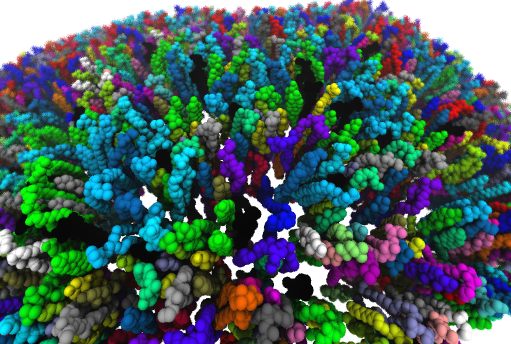
\includegraphics{content/images/membrane-vmd.png}
\caption{\DIFadd{An example of a curved membrane with many different lipid
species, colored separately, representative of the systems I will
simulate.}}
\label{fig:membrane-setup}
\end{wrapfloat}

\DIFadd{Despite advances in super-resolution microscopy, such as PALM and STORM,
}\emph{\DIFadd{in vivo}} \DIFadd{characterization of membrane heterogeneity remains
challenging due to the high spatiotemporal resolution required to study
fluctuating nanoscale assemblies of lipids and proteins in living cells.
However, a variety of indirect experimental techniques, often using
fluorescently labeled lipid analogs, have characterized the existence of
sub-micron sized domains in living cells and plasma membrane
extracts\textsuperscript{\protect\hyperlink{ref-GGtK2c0N}{28}--\protect\hyperlink{ref-aiu6Tmil}{32}}.
Even in the absence of proteins, }\emph{\DIFadd{in vitro}} \DIFadd{assays in the Janmey
group have demonstrated clusters of negatively charged phospholipids of
on the order of 50 nm after the addition of as little as 1 μM
Ca\textsuperscript{2+}\textsuperscript{\protect\hyperlink{ref-LhOwGz4k}{23}}.
}

\DIFadd{My approach is to understand what conditions promote cluster formation
and how the behavior of lipids in clusters differs from bulk. I will
initially focus on delineating the nucleation of cation-induced clusters
of anionic phospholipids. This work will involve extending the methods I
developed to investigate single molecule QM/MM and all-atom nanoscale
simulations. In those simulations, I found that Ca\textsuperscript{2+}
can act as ``molecular glue,'' forming aggregates of three lipids that
remain together for at least 100 ns, much longer than other ion-lipid
bond lifetimes. Extending beyond the all-atom simulations, I will use
the }\href{https://github.com/biophyscode}{methods} \DIFadd{we created to
construct and equilibrate multi-component membrane systems to build
models containing rich mixtures of phospholipids (Figure
\ref{fig:membrane-setup}), going past typical two or three-component
systems that are frequently used.
}

\DIFadd{The finite and well-defined size of the domains suggests there is a
balance between the mutual electrostatic and steric repulsion of
negatively charged lipids and attraction mediated by counterions. I will
monitor the extent of phase separation and demixing in simulations
containing combinations of physiological divalent and monovalent ions
with varying fractions of charged and uncharged lipids. The calculated
diffusion coefficient inside the clusters can be compared with values
obtained using fluorescence correlation spectroscopy (FCS) and spot
variant FCS\textsuperscript{\protect\hyperlink{ref-oBaB5Z87}{30}}.
Simple, physical models based primarily on
electrostatics\textsuperscript{\protect\hyperlink{ref-10CqL9t0a}{33}}
predict continual growth of clusters in the presence of excess
counterions, yet }\emph{\DIFadd{in vivo}} \DIFadd{clusters plateau at a stable size. By
using coarse-grained simulations and GPU-accelerated molecular dynamics,
I will be able to study the growth and merging of clusters on the
microsecond to millisecond timescale. The size and shape of the
simulated clusters will be contrasted with those seen with AFM imaging
and electron
microscopy\textsuperscript{\protect\hyperlink{ref-LhOwGz4k}{23}}.
}

\DIFadd{Experiments pulling thin membrane tethers have shown that
phase-separated phospholipid domains form precisely at the junction of
highly curved
regions\textsuperscript{\protect\hyperlink{ref-XIltXoGI}{34}}, implying
a relationship between membrane morphology an lipid sorting. I will
compare the bending modulus and mean curvature of clusters with data
from pipette aspiration of membrane
tubules\textsuperscript{\protect\hyperlink{ref-oBaB5Z87}{30},\protect\hyperlink{ref-aiu6Tmil}{32},\protect\hyperlink{ref-XIltXoGI}{34}}.
The order parameter of lipids in and on the boundary of the cluster can
be compared to results complementary non-fluorescent methods, such as
EPR, NMR, and neutron scattering.
}


\begin{wrapfloat}{figure}{L}{2in}
\centering
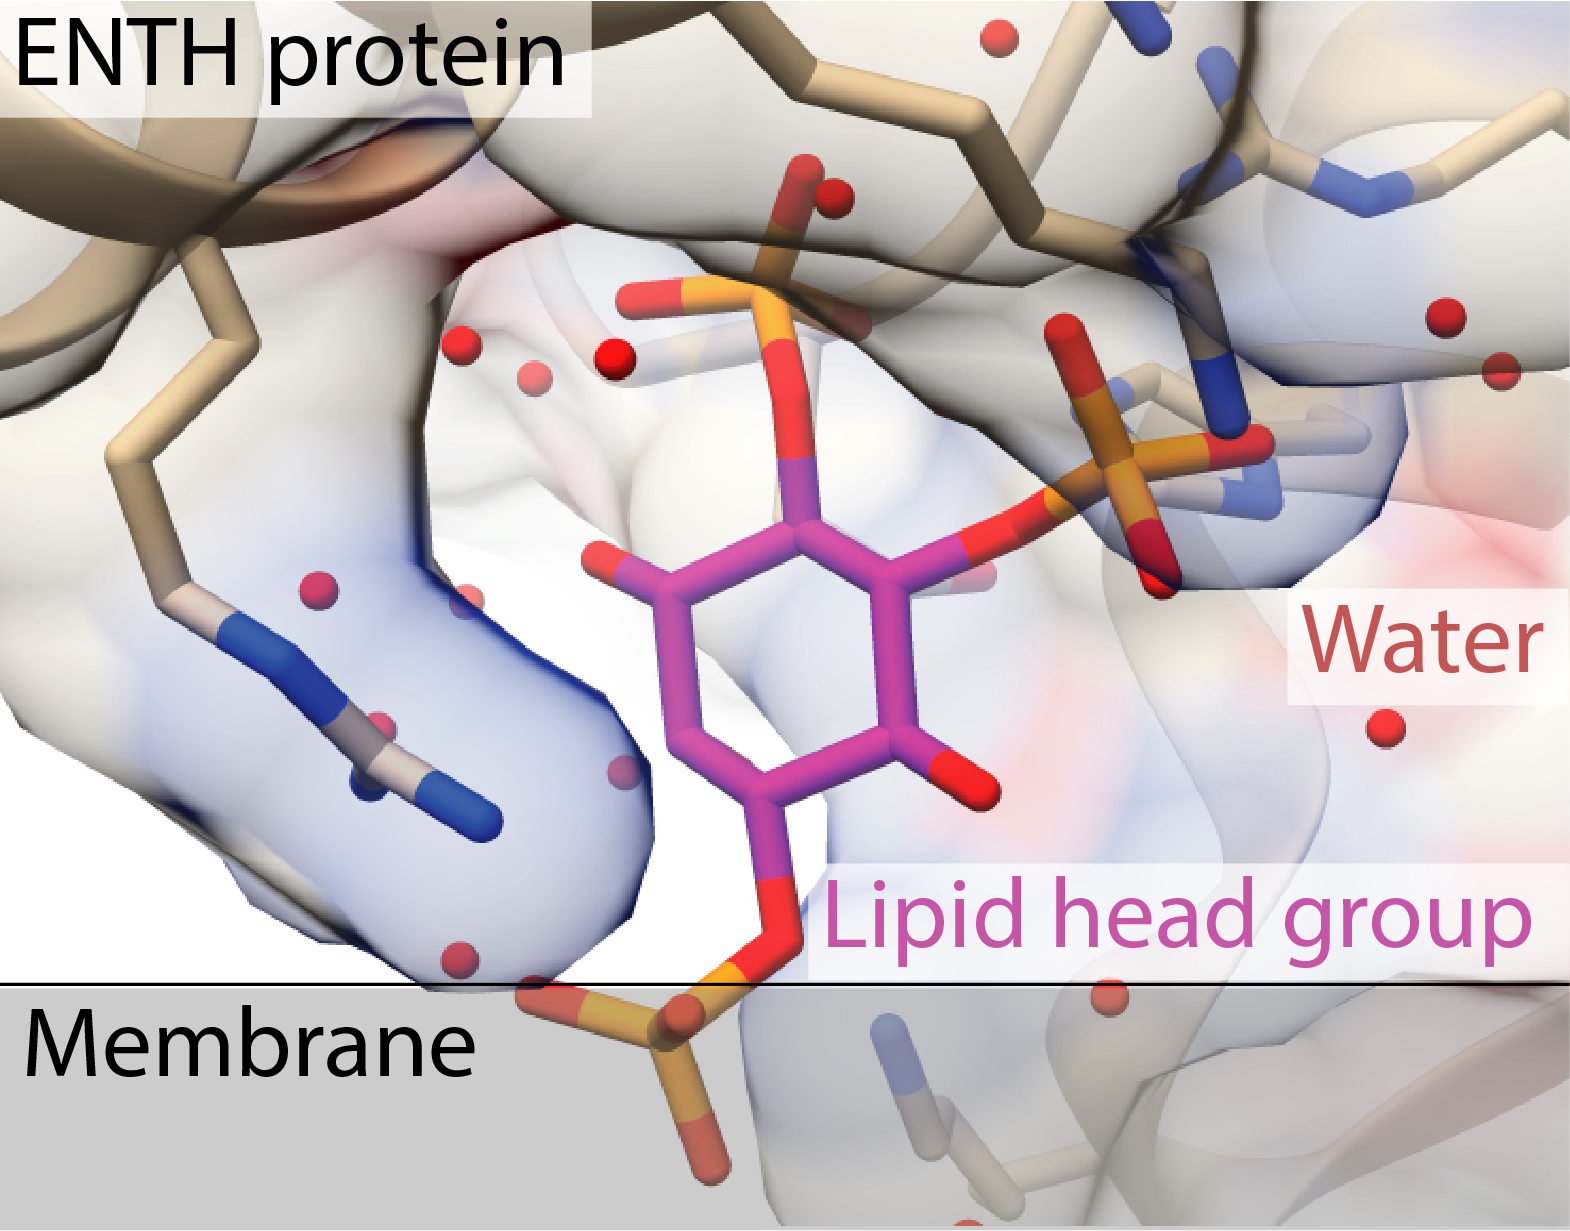
\includegraphics{content/images/stereospecific.png}
\caption{\DIFadd{An illustration of stereospecific recognition of phospholipids
by proteins.}}
\label{fig:stereospecific}
\end{wrapfloat}

\DIFadd{Finally, I will study whether the act of being in a cluster alters the
ability of certain lipids to perform their biological roles. Many of the
lipids implicated in cluster formation, such as
PtdIns(4,5)}\emph{\DIFadd{P}}\DIFadd{\textsubscript{2}, have been shown to bind hundreds
of proteins\textsuperscript{\protect\hyperlink{ref-uyKE7bWV}{16}}, and
several integral membrane proteins have been shown to partition into
lipid raft-like
domains\textsuperscript{\protect\hyperlink{ref-2TfZ4zWV}{35}}.
PtdIns(4,5)}\emph{\DIFadd{P}}\DIFadd{\textsubscript{2} binds (some) proteins in a highly
stereospecific manner (Figure \ref{fig:stereospecific}) requiring a
fully extended and accessible head group. In order to evaluate the
biological consequences of clustering, I will run simulations containing
proteins that bind through either non-specific, electrostatic attraction
(e.g., N-WASP and gelsolin) or through tight coordination (e.g., the PH
domain of PLCδ. I will test whether these proteins bind ``free'' lipid
molecules as well as they bind clustered ones by using steered molecular
dynamics.
}

\DIFadd{I expect the outcome of studying domain formation to be especially
helpful for building better models of plasma membranes that reflect the
complex cellular environment. I anticipate these results could provide a
quantitative insights for pore-formation in cell membranes by toxins and
cationic surfactants, the activation of integral ion channels and GPCRs
by PtdIns(4,5)}\emph{\DIFadd{P}}\DIFadd{\textsubscript{2}, and the dynamics of membrane
fusion, fission and other buckling geometries.
}

\DIFaddend \hypertarget{what-are-the-mechanical-properties-of-synthetic-molecular-motors}{%
\subsection{What are the mechanical properties of synthetic molecular
motors?}\label{what-are-the-mechanical-properties-of-synthetic-molecular-motors}}


\begin{wrapfloat}{figure}{L}{2in}
\centering
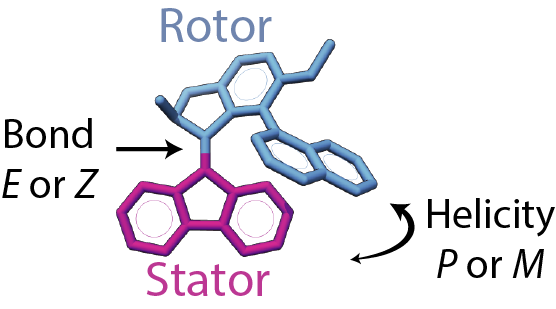
\includegraphics{content/images/motor.png}
\caption{The two degrees of freedom in a synthetic molecular motor.}
\label{fig:motor-diagram}
\end{wrapfloat}

The ability of light-driven molecular motors to switch between two or
more states makes them suitable for new forms of optical data
storage\textsuperscript{\protect\DIFdelbegin %DIFDELCMD < \hyperlink{ref-18PGyWtWV}{28}%%%
\DIFdelend \DIFaddbegin \hyperlink{ref-18PGyWtWV}{36}\DIFaddend }, as
``wheels'' on nano-scale
cars\textsuperscript{\protect\DIFdelbegin %DIFDELCMD < \hyperlink{ref-OAnfwOYX}{29}%%%
\DIFdelend \DIFaddbegin \hyperlink{ref-OAnfwOYX}{37}\DIFaddend },
trains\textsuperscript{\protect\DIFdelbegin %DIFDELCMD < \hyperlink{ref-10MPrT2Vf}{30}%%%
\DIFdelend \DIFaddbegin \hyperlink{ref-10MPrT2Vf}{38}\DIFaddend },
worms\textsuperscript{\protect\DIFdelbegin %DIFDELCMD < \hyperlink{ref-Tels98bO}{31}%%%
\DIFdelend \DIFaddbegin \hyperlink{ref-Tels98bO}{39}\DIFaddend }, and
walkers\textsuperscript{\protect\DIFdelbegin %DIFDELCMD < \hyperlink{ref-SfUEsk0e}{32}%%%
\DIFdelend \DIFaddbegin \hyperlink{ref-SfUEsk0e}{40}\DIFaddend }, or in new
forms of responsive
materials\textsuperscript{\protect\DIFdelbegin %DIFDELCMD < \hyperlink{ref-jCuccJLJ}{33}%%%
\DIFdelend \DIFaddbegin \hyperlink{ref-jCuccJLJ}{41}\DIFaddend }. Unlike
switches, whose work is reversed after every full cycle, molecular
motors can be used to progressively move systems away from thermodynamic
equilibrium\textsuperscript{\protect\DIFdelbegin %DIFDELCMD < \hyperlink{ref-1H5r7SBir}{34}%%%
\DIFdelend \DIFaddbegin \hyperlink{ref-1H5r7SBir}{42}\DIFaddend }. The
synthetic molecular motors of Ben Fergina operate by converting light
and heat into directional rotary motion. These motors belong to a class
of molecules called overcrowded alkenes, with two stable enantiomers,
and adopt a helical shape due to steric strain around the central double
bond. The two sets of conjugated rings rotate relative to each other,
with the central bond acting as an axle, and for simplicity, one set of
rings is designated the ``stator'' while the other set is called the
``rotor.'' The directional motion of these molecules can be analyzed in
terms of two degrees of freedom: \(E\) to \(Z\) for the isomerization of
the double bond (analogous to \emph{cis} and \emph{trans}) and \(P\) and
\(M\) for the overall twist or helicity of the molecule (Figure
\ref{fig:motor-diagram}).

\hypertarget{calculate-the-speed-torque-and-efficiency-of-motors}{%
\subsubsection{Calculate the speed, torque, and efficiency of
motors}\label{calculate-the-speed-torque-and-efficiency-of-motors}}

In 2006, it was shown that light driven molecular motors can rotate a
glass rod that is more than 10,000 times their size upon irradiation
with light and when included as a dopant in a liquid crystal
film\textsuperscript{\protect\DIFdelbegin %DIFDELCMD < \hyperlink{ref-thFGBz32}{35}%%%
\DIFdelend \DIFaddbegin \hyperlink{ref-thFGBz32}{43}\DIFaddend }. While it is
clear that artificial motors, when aligned appropriately so their
individual effects are magnified, can produce macroscopic effects, it is
not known how much force an individual molecular motor can generate. I
will take the nonequilibrium model I developed to quantify directional
motion in biological motors to these artificial molecular motors, in a
new direction, focusing on the ``second generation'' class of motors
from Ben Feringa and colleagues, which possess chemically symmetric
stators and a lower energy for the thermal step. I will study the four
ground states that comprise the 360\(^\circ\) cycle depicted in Figure
\ref{fig:motors}. On the left, the four structural states of the motor
demonstrate movement of the upper rotor relative to the fixed stator
through two photochemical (\(1 \rightarrow 2, 3 \rightarrow 4\)) and two
thermal steps (\(2 \rightarrow 3, 4 \rightarrow 1\)). On the right, I've
sketched illustrative free energy profiles along a given surface \(E\)
or \(Z\); these represent the pattern of energy troughs and barriers for
changing the helicity of the structure while maintaining the same
orientation of the double bond, essentially sliding the bulky biaryl
rings connected to the rotor past the stator.

\begin{figure}
\centering
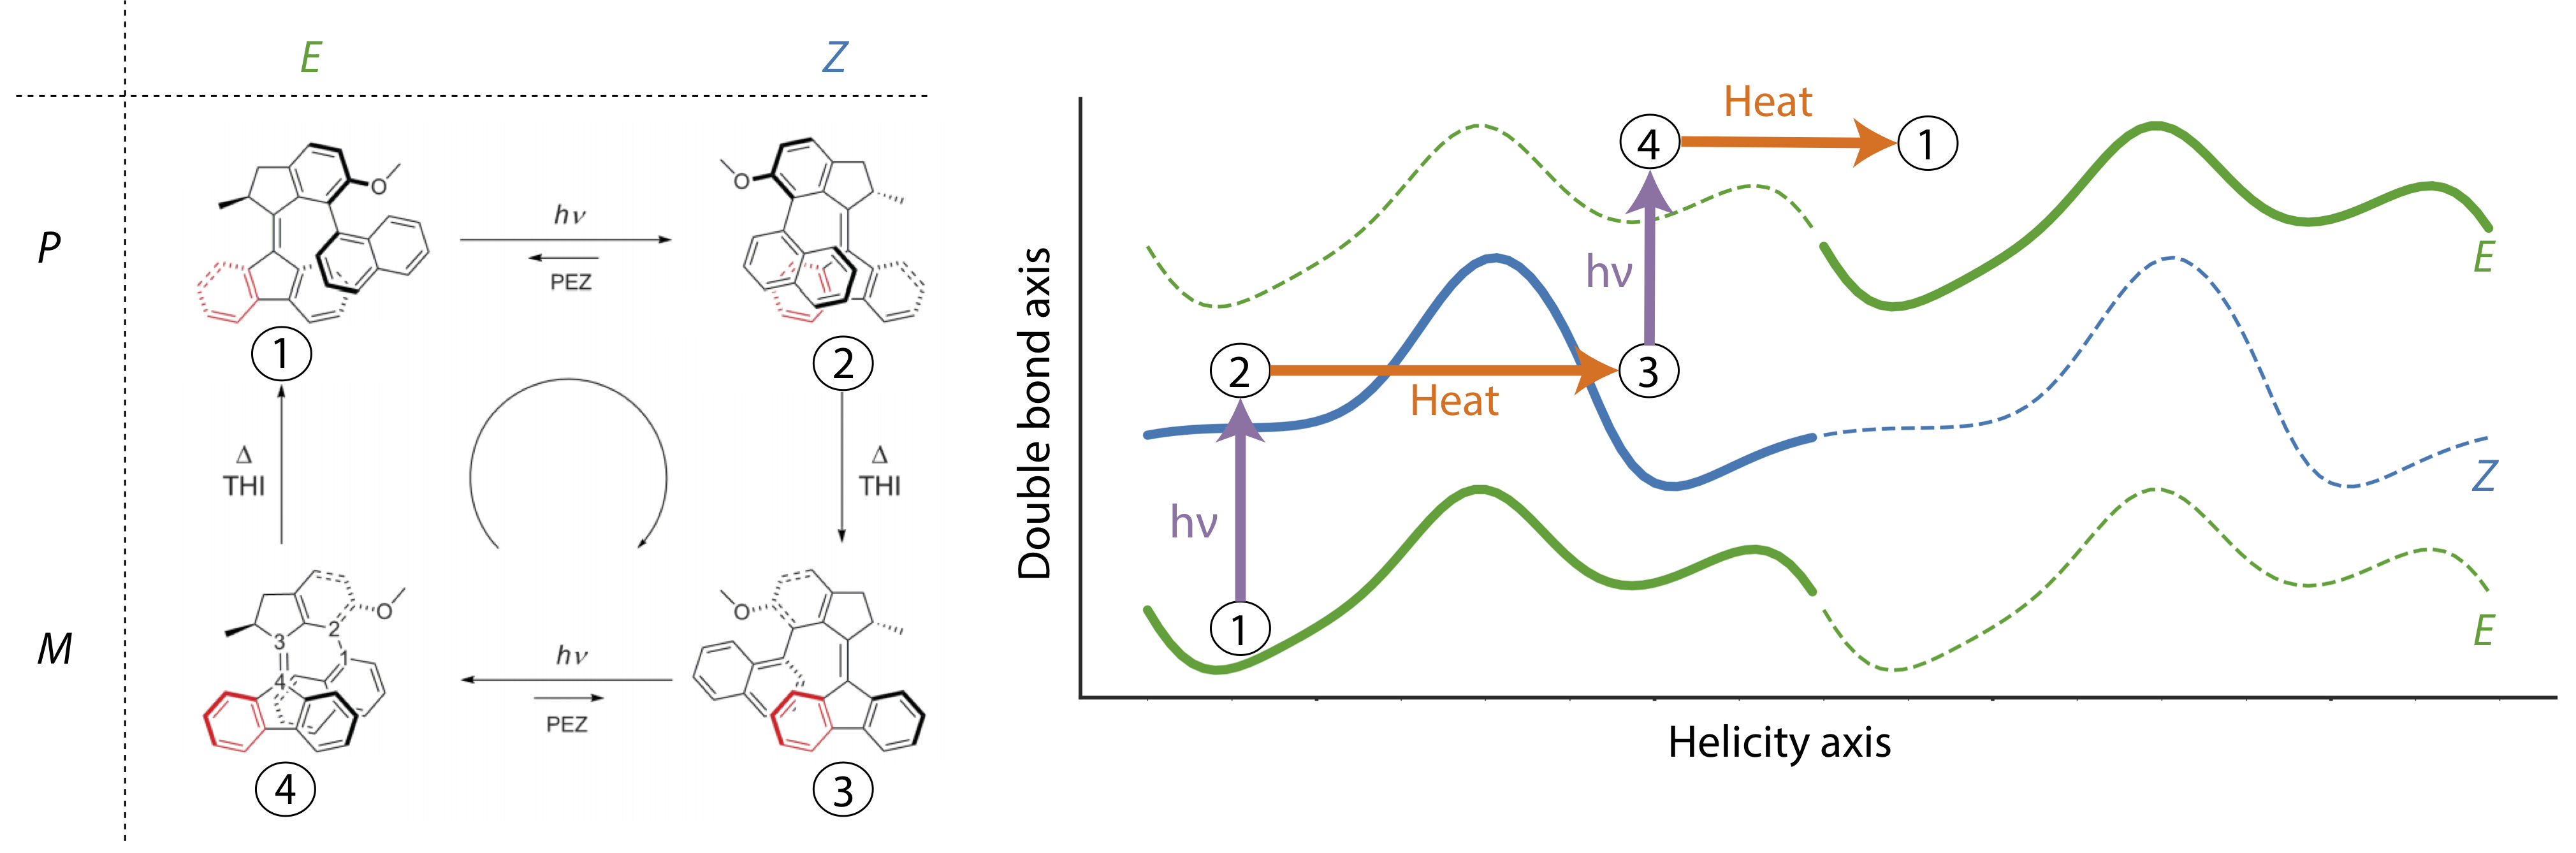
\includegraphics[width=1\textwidth,height=\textheight]{content/images/offset-barriers.png}
\caption{On the left, the four ground state conformations of a second
generation motor, adapted from Štacko et
al\DIFdelbeginFL \DIFdelFL{\textsuperscript{\protect\hyperlink{ref-mKSNFvW7}{36}}}\DIFdelendFL \DIFaddbeginFL \DIFaddFL{\textsuperscript{\protect\hyperlink{ref-mKSNFvW7}{44}}}\DIFaddendFL . On the right,
the same four states placed on free energy profiles. The energy profiles
are periodic, with two cycles shown for both isomerization state. A
clone of the lower \(E\) energy surface is shown above, for clarity, to
demonstrate the progression from state 4 to state 1 requires
energy.\label{fig:motors}}
\end{figure}

Previously we used microsecond-scale molecular dynamics simulations to
determine the energy landscapes based on equilibrium population
distributions. However, because the barriers here are expected to be
much larger, I will directly probe the potential surfaces by evaluating
the energy of motor conformations for different values of the central
dihedral angle. I will perform this dihedral scan using a quantum
chemistry package, such as \href{http://psicode.org/}{Psi4} with density
functional theory and semi-empirical methods. I will begin with the
semi-empirical methods PM3 or AM1 and test the sensitivity of the
results to different quantum approaches (e.g., other types of DFT and
Hartree-Fock) and basis sets (e.g., 6-31G*). From the discrete free
energy profiles, the rate of bin-to-bin transitions can be deduced, and
these are gathered, together with the surface-to-surface transition
rates, in a Markov matrix. Solving for the eigenvectors of the matrix
yields the nonequilibrium steady state (NESS) population in each
photochemical state of the motor. From the NESS, I will calculate the
net probability flux for the complete cycle (\(1 \rightarrow 1\)), as
illustrated by the series of purple and orange arrows in Figure
\ref{fig:motors}, for a given input level of light irradiation.

\hypertarget{optimize-the-design-of-artificial-molecular-motors}{%
\subsubsection{Optimize the design of artificial molecular
motors}\label{optimize-the-design-of-artificial-molecular-motors}}

As demonstrated by Richard Feynman in a lecture on Brownian ratchets,
the challenge of designing molecular motors is not how to create
movement, but how to control the directionality of the omnipresent --
and random -- motion on the molecular
scale\textsuperscript{\protect\DIFdelbegin %DIFDELCMD < \hyperlink{ref-10FsKpWBI}{37}%%%
\DIFdelend \DIFaddbegin \hyperlink{ref-10FsKpWBI}{45}\DIFaddend }. This has
been referred to as the ``gating'' of stochastic
motion\textsuperscript{\protect\DIFdelbegin %DIFDELCMD < \hyperlink{ref-qhUBHBOM}{38}%%%
\DIFdelend \DIFaddbegin \hyperlink{ref-qhUBHBOM}{46}\DIFaddend }. In my
previous work\textsuperscript{\protect\hyperlink{ref-1BfYw0gk2}{3}}, I
showed that the gating can arise purely from the complementary shape of
two potential energy surfaces, whereby an unpassable barrier on one
surface can be circumnavigated by motion on the other surface (see
Figure S6, in particular.) In this section, I will explore the
relationship between the shape of the potential energy surfaces and the
directionality of artificial molecular motors. This sub-aim will test
the current understanding of motor mechanisms, most of which has been
inferred through static structural snapshots and chemical intuition,
using design proofs and will open the field of rational design to
molecular rotors, pumps, transporters, and other nanorobotics.

It has been empirically determined that adding electron donating and
electron withdrawing moieties has the potential to affect the rotation
rate of the
motor\textsuperscript{\protect\DIFdelbegin %DIFDELCMD < \hyperlink{ref-1AzLiBVkC}{39}%%%
\DIFdelend \DIFaddbegin \hyperlink{ref-1AzLiBVkC}{47}\DIFaddend }. Polarizing
the molecule by placing electron withdrawing and electron donating
groups on either end of the central double bond, has the potential to
lengthen the effective axle, significantly reducing the barrier for
rotation. I will numerically optimize the potential energy surfaces that
I determine in the previous sub-aim, to yield the maximum directional
flux and maximum torque (see Figure \ref{fig:COBYLA} for an example).
The surfaces will be modeled as splines with six to eight control points
evenly spaced along the periodic degree of freedom and the spline points
will be allowed to move as the optimization procedure runs. Based on
preliminary work, this procedure affords ample room to significantly
change the properties of the surfaces. I will couple the understanding
that arises from this study with the knowledge of how chemical
constituents affect overall rotation rates to suggest new avenues for
synthetic motor design.

\begin{figure}
\centering
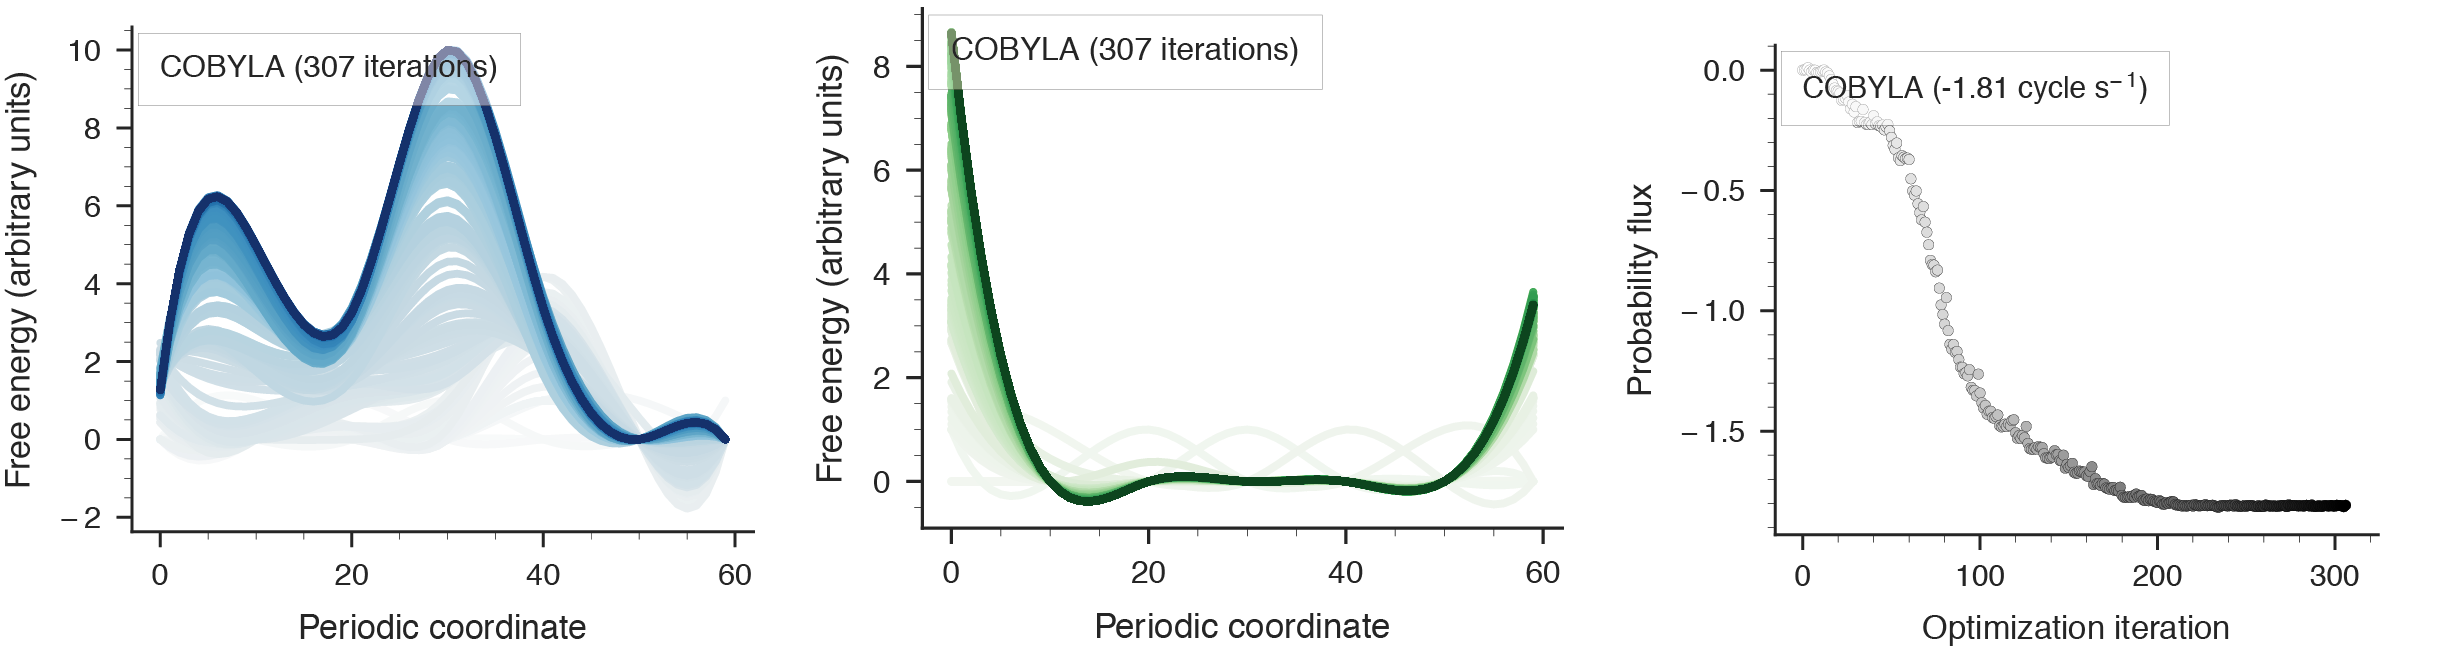
\includegraphics[width=1\textwidth,height=\textheight]{content/images/COBYLA.png}
\caption{Example optimization (using the constrained optimization by
linear approximation algorithm, COBYLA) of motor surfaces for maximum
flux. Later iterations are darker colors. On the left, the \(Z\)
surface; in the middle, the \(E\) surface; on the right, the net
probability flux corresponding to each optimization
iteration.\label{fig:COBYLA}}
\end{figure}

\DIFaddbegin \hypertarget{develop-a-physical-theory-of-molecular-motors}{%
\subsection{Develop a physical theory of molecular
motors}\label{develop-a-physical-theory-of-molecular-motors}}

\DIFadd{\textcolor{Maroon}{The proposed research the mechanical properties of existing synthetic molecular motors and suggest new design routes for future nanomachines.}
}


\begin{wrapfloat}{figure}{L}{2in}
\centering
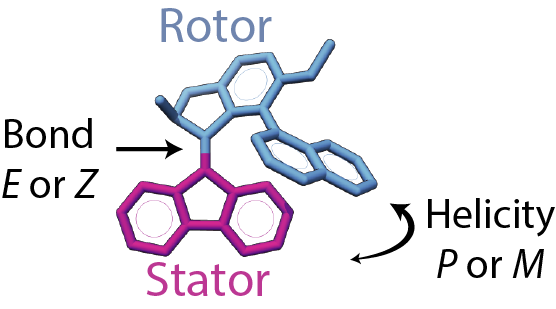
\includegraphics{content/images/motor.png}
\caption{\DIFadd{The two degrees of freedom in a synthetic molecular motor.}}
\label{fig:motor-diagram}
\end{wrapfloat}

\DIFadd{The ability of light-driven molecular motors to switch between two or
more states makes them suitable for new forms of optical data
storage\textsuperscript{\protect\hyperlink{ref-18PGyWtWV}{36}}, as
``wheels'' on nano-scale
cars\textsuperscript{\protect\hyperlink{ref-OAnfwOYX}{37}},
trains\textsuperscript{\protect\hyperlink{ref-10MPrT2Vf}{38}},
worms\textsuperscript{\protect\hyperlink{ref-Tels98bO}{39}}, and
walkers\textsuperscript{\protect\hyperlink{ref-SfUEsk0e}{40}}, or in new
forms of responsive
materials\textsuperscript{\protect\hyperlink{ref-jCuccJLJ}{41}}. Unlike
switches, whose work is reversed after every full cycle, molecular
motors can be used to progressively move systems away from thermodynamic
equilibrium\textsuperscript{\protect\hyperlink{ref-1H5r7SBir}{42}}. The
synthetic molecular motors of Ben Fergina operate by converting light
and heat into directional rotary motion. These motors belong to a class
of molecules called overcrowded alkenes, with two stable enantiomers,
and adopt a helical shape due to steric strain around the central double
bond. The two sets of conjugated rings rotate relative to each other,
with the central bond acting as an axle, and for simplicity, one set of
rings is designated the ``stator'' while the other set is called the
``rotor.'' The directional motion of these molecules can be analyzed in
terms of two degrees of freedom: \(E\) to \(Z\) for the isomerization of
the double bond (analogous to }\emph{\DIFadd{cis}} \DIFadd{and }\emph{\DIFadd{trans}}\DIFadd{) and \(P\) and
\(M\) for the overall twist or helicity of the molecule (Figure
\ref{fig:motor-diagram}).
}

\hypertarget{calculate-the-speed-torque-and-efficiency-of-motors-1}{%
\subsubsection{Calculate the speed, torque, and efficiency of
motors}\label{calculate-the-speed-torque-and-efficiency-of-motors-1}}

\DIFadd{In 2006, it was shown that light driven molecular motors can rotate a
glass rod that is more than 10,000 times their size upon irradiation
with light and when included as a dopant in a liquid crystal
film\textsuperscript{\protect\hyperlink{ref-thFGBz32}{43}}. While it is
clear that artificial motors, when aligned appropriately so their
individual effects are magnified, can produce macroscopic effects, it is
not known how much force an individual molecular motor can generate. I
will take the nonequilibrium model I developed to quantify directional
motion in biological motors to these artificial molecular motors, in a
new direction, focusing on the ``second generation'' class of motors
from Ben Feringa and colleagues, which possess chemically symmetric
stators and a lower energy for the thermal step. I will study the four
ground states that comprise the 360\(^\circ\) cycle depicted in Figure
\ref{fig:motors}. On the left, the four structural states of the motor
demonstrate movement of the upper rotor relative to the fixed stator
through two photochemical (\(1 \rightarrow 2, 3 \rightarrow 4\)) and two
thermal steps (\(2 \rightarrow 3, 4 \rightarrow 1\)). On the right, I've
sketched illustrative free energy profiles along a given surface \(E\)
or \(Z\); these represent the pattern of energy troughs and barriers for
changing the helicity of the structure while maintaining the same
orientation of the double bond, essentially sliding the bulky biaryl
rings connected to the rotor past the stator.
}

\begin{figure}
\centering
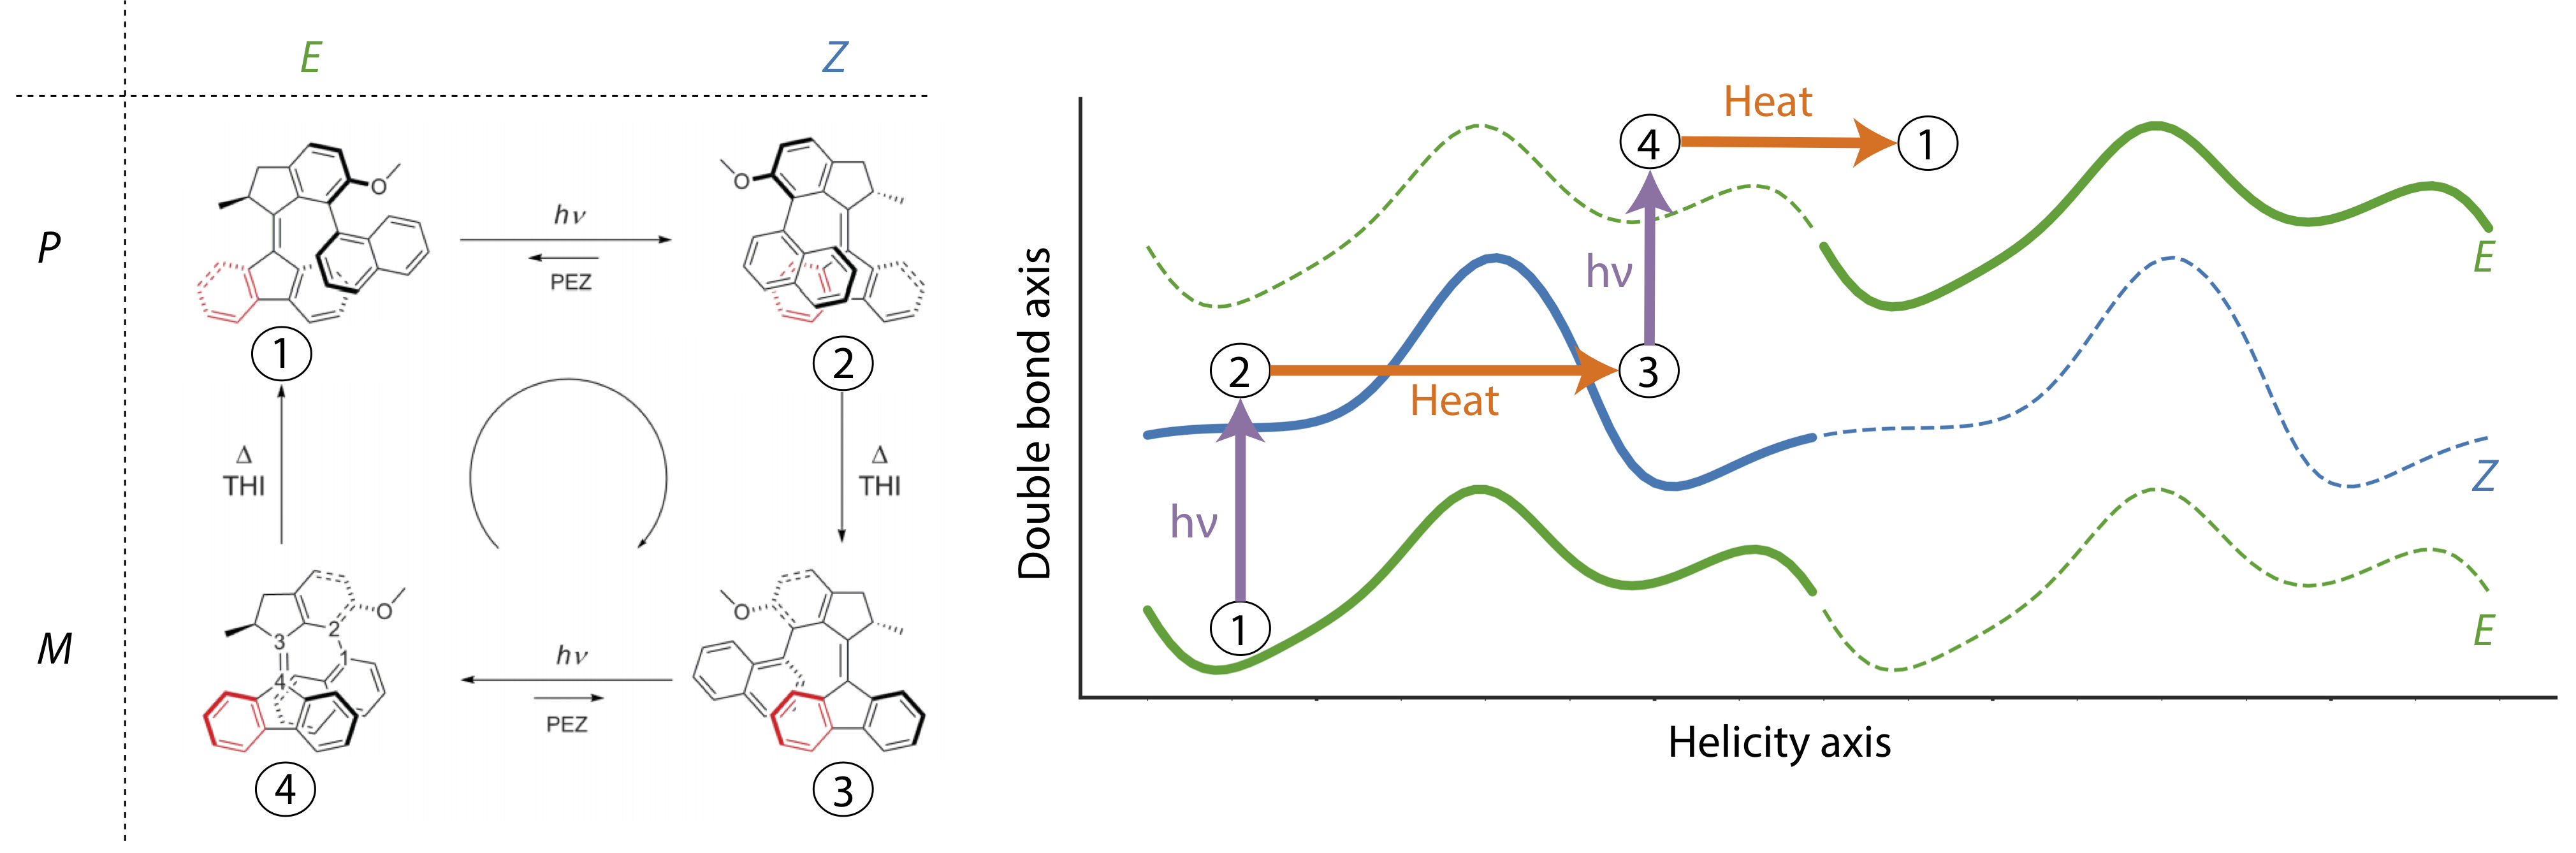
\includegraphics[width=1\textwidth,height=\textheight]{content/images/offset-barriers.png}
\caption{\DIFaddFL{On the left, the four ground state conformations of a second
generation motor, adapted from Štacko et
al\textsuperscript{\protect\hyperlink{ref-mKSNFvW7}{44}}. On the right,
the same four states placed on free energy profiles. The energy profiles
are periodic, with two cycles shown for both isomerization state. A
clone of the lower \(E\) energy surface is shown above, for clarity, to
demonstrate the progression from state 4 to state 1 requires
energy.}\label{fig:motors}}
\end{figure}

\DIFadd{Previously we used microsecond-scale molecular dynamics simulations to
determine the energy landscapes based on equilibrium population
distributions. However, because the barriers here are expected to be
much larger, I will directly probe the potential surfaces by evaluating
the energy of motor conformations for different values of the central
dihedral angle. I will perform this dihedral scan using a quantum
chemistry package, such as }\href{http://psicode.org/}{Psi4} \DIFadd{with density
functional theory and semi-empirical methods. I will begin with the
semi-empirical methods PM3 or AM1 and test the sensitivity of the
results to different quantum approaches (e.g., other types of DFT and
Hartree-Fock) and basis sets (e.g., 6-31G*). From the discrete free
energy profiles, the rate of bin-to-bin transitions can be deduced, and
these are gathered, together with the surface-to-surface transition
rates, in a Markov matrix. Solving for the eigenvectors of the matrix
yields the nonequilibrium steady state (NESS) population in each
photochemical state of the motor. From the NESS, I will calculate the
net probability flux for the complete cycle (\(1 \rightarrow 1\)), as
illustrated by the series of purple and orange arrows in Figure
\ref{fig:motors}, for a given input level of light irradiation.
}

\hypertarget{optimize-the-design-of-artificial-molecular-motors-1}{%
\subsubsection{Optimize the design of artificial molecular
motors}\label{optimize-the-design-of-artificial-molecular-motors-1}}

\DIFadd{As demonstrated by Richard Feynman in a lecture on Brownian ratchets,
the challenge of designing molecular motors is not how to create
movement, but how to control the directionality of the omnipresent --
and random -- motion on the molecular
scale\textsuperscript{\protect\hyperlink{ref-10FsKpWBI}{45}}. This has
been referred to as the ``gating'' of stochastic
motion\textsuperscript{\protect\hyperlink{ref-qhUBHBOM}{46}}. In my
previous work\textsuperscript{\protect\hyperlink{ref-1BfYw0gk2}{3}}, I
showed that the gating can arise purely from the complementary shape of
two potential energy surfaces, whereby an unpassable barrier on one
surface can be circumnavigated by motion on the other surface (see
Figure S6, in particular.) In this section, I will explore the
relationship between the shape of the potential energy surfaces and the
directionality of artificial molecular motors. This sub-aim will test
the current understanding of motor mechanisms, most of which has been
inferred through static structural snapshots and chemical intuition,
using design proofs and will open the field of rational design to
molecular rotors, pumps, transporters, and other nanorobotics.
}

\DIFadd{It has been empirically determined that adding electron donating and
electron withdrawing moieties has the potential to affect the rotation
rate of the
motor\textsuperscript{\protect\hyperlink{ref-1AzLiBVkC}{47}}. Polarizing
the molecule by placing electron withdrawing and electron donating
groups on either end of the central double bond, has the potential to
lengthen the effective axle, significantly reducing the barrier for
rotation. I will numerically optimize the potential energy surfaces that
I determine in the previous sub-aim, to yield the maximum directional
flux and maximum torque (see Figure \ref{fig:COBYLA} for an example).
The surfaces will be modeled as splines with six to eight control points
evenly spaced along the periodic degree of freedom and the spline points
will be allowed to move as the optimization procedure runs. Based on
preliminary work, this procedure affords ample room to significantly
change the properties of the surfaces. I will couple the understanding
that arises from this study with the knowledge of how chemical
constituents affect overall rotation rates to suggest new avenues for
synthetic motor design.
}

\begin{figure}
\centering
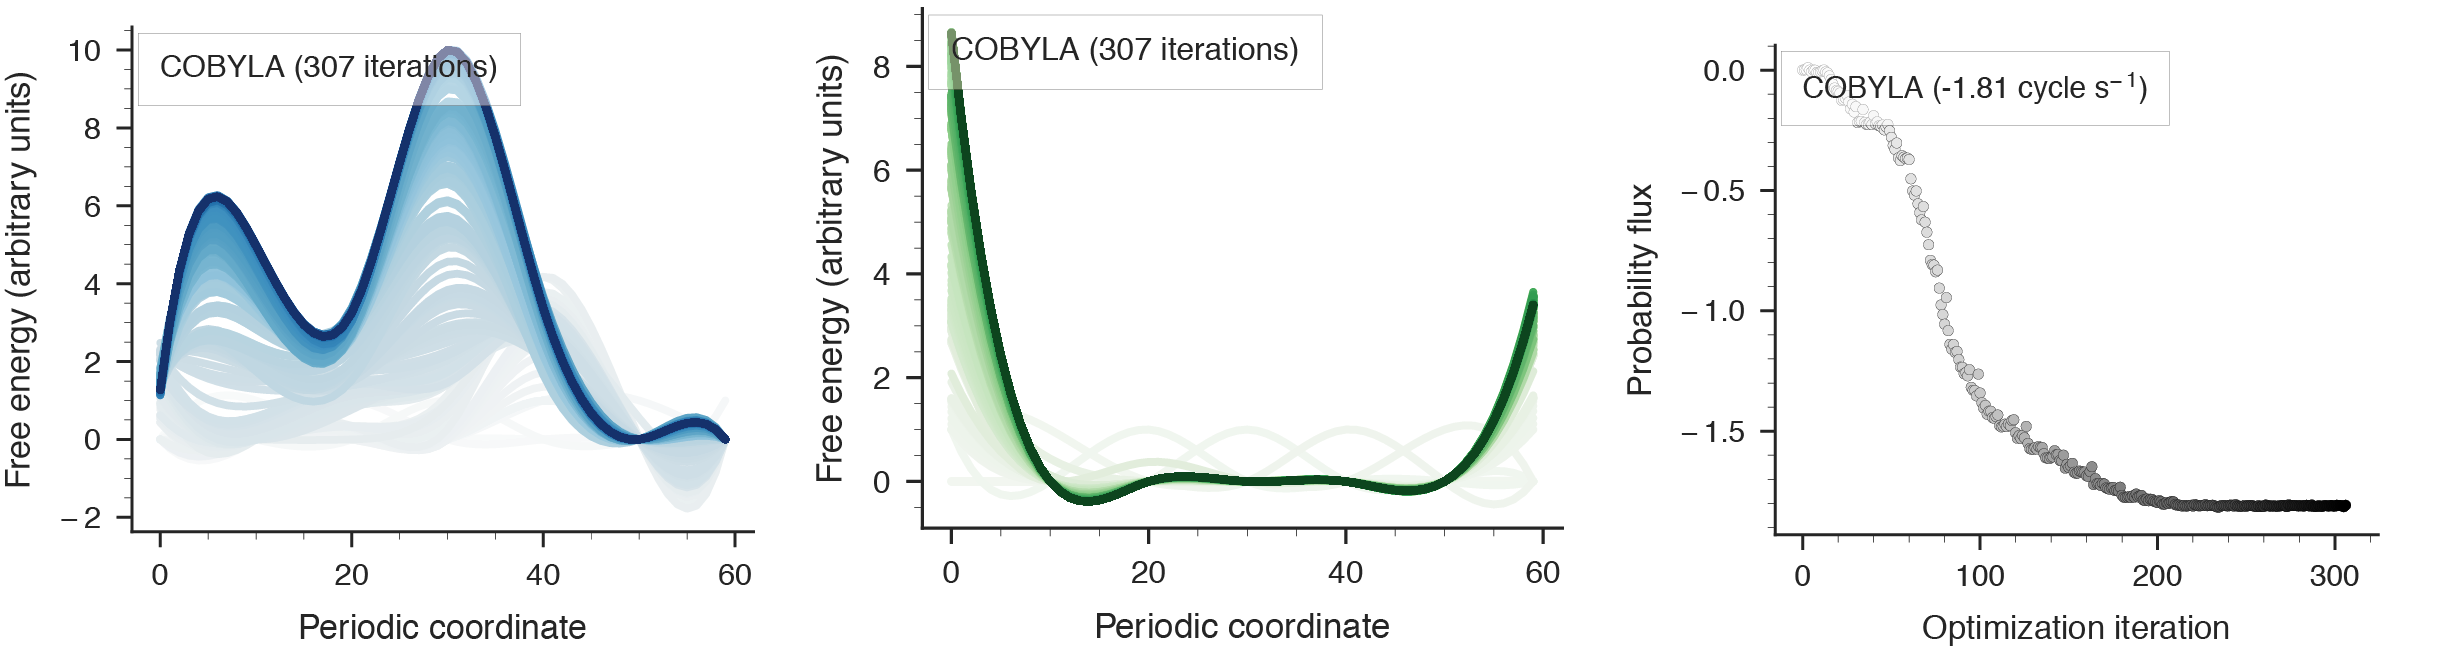
\includegraphics[width=1\textwidth,height=\textheight]{content/images/COBYLA.png}
\caption{\DIFaddFL{Example optimization (using the constrained optimization by
linear approximation algorithm, COBYLA) of motor surfaces for maximum
flux. Later iterations are darker colors. On the left, the \(Z\)
surface; in the middle, the \(E\) surface; on the right, the net
probability flux corresponding to each optimization
iteration.}\label{fig:COBYLA}}
\end{figure}

\DIFaddend \hypertarget{building-better-force-fields-for-drug-discovery-using-open-data-and-automated-optimization}{%
\subsection{Building better force fields for drug discovery using open
data and automated
optimization}\label{building-better-force-fields-for-drug-discovery-using-open-data-and-automated-optimization}}

Designing ligands that bind their target with high affinity and
specificity is the principal objective of small-molecule drug discovery,
yet hit-to-lead and lead-optimization can take upwards of three years
owing to the fact it is often necessary to synthesize hundreds or
thousands of new compounds. In short, drug discovery is very expensive
and often fails. In recent years, the pharmaceutical industry has begun
to use absolute and relative binding free energy calculations to help
narrow the number of compounds that must be
synthesized\textsuperscript{\protect\DIFdelbegin %DIFDELCMD < \hyperlink{ref-1FiDpP1LR}{40}%%%
\DIFdelend \DIFaddbegin \hyperlink{ref-1FiDpP1LR}{48}\DIFaddend ,\protect\DIFdelbegin %DIFDELCMD < \hyperlink{ref-1BwXH3GFO}{41}%%%
\DIFdelend \DIFaddbegin \hyperlink{ref-1BwXH3GFO}{49}\DIFaddend }.
In particular, the advent of computational calorimetry has enabled
quantitative and high-precision comparisons of binding free energies,
enthalpies, and entropies (by subtraction) with experimental values
determined by isothermal titration calorimetry or
NMR\textsuperscript{\protect\DIFdelbegin %DIFDELCMD < \hyperlink{ref-1935a9V0d}{42}%%%
\DIFdelend \DIFaddbegin \hyperlink{ref-1935a9V0d}{50}\DIFaddend }. The root
mean squared error (RMSE) associated with such calculations is in the
range of 1-4
kcal/mol\textsuperscript{\protect\DIFdelbegin %DIFDELCMD < \hyperlink{ref-LWd10vQy}{43}%%%
\DIFdelend \DIFaddbegin \hyperlink{ref-LWd10vQy}{51}\DIFaddend }, yet even
a modest improvement of the prediction accuracy of \textasciitilde{}1
kcal/mol would lead to a substantial decrease in the number of compounds
that must be manually screened by nearly an order of
magnitude\textsuperscript{\protect\DIFdelbegin %DIFDELCMD < \hyperlink{ref-fC0t6Cy1}{44}%%%
\DIFdelend \DIFaddbegin \hyperlink{ref-fC0t6Cy1}{52}\DIFaddend }.
Although it has been suggested by some that changes in the force field
functional form are required, it is clear that there is ample room to
improve the accuracy of existing parameters through careful
analysis\textsuperscript{\protect\DIFdelbegin %DIFDELCMD < \hyperlink{ref-LOjcxYqt}{45}%%%
\DIFdelend \DIFaddbegin \hyperlink{ref-LOjcxYqt}{53}\DIFaddend }. The
first goal of this aim is to create better tools to guide early-stage
drug discovery by reducing the number of compounds that must be
synthesized to find a promising hit that can be carried over into
clinical trials.


\begin{wrapfloat}{figure}{L}{3in}
\centering
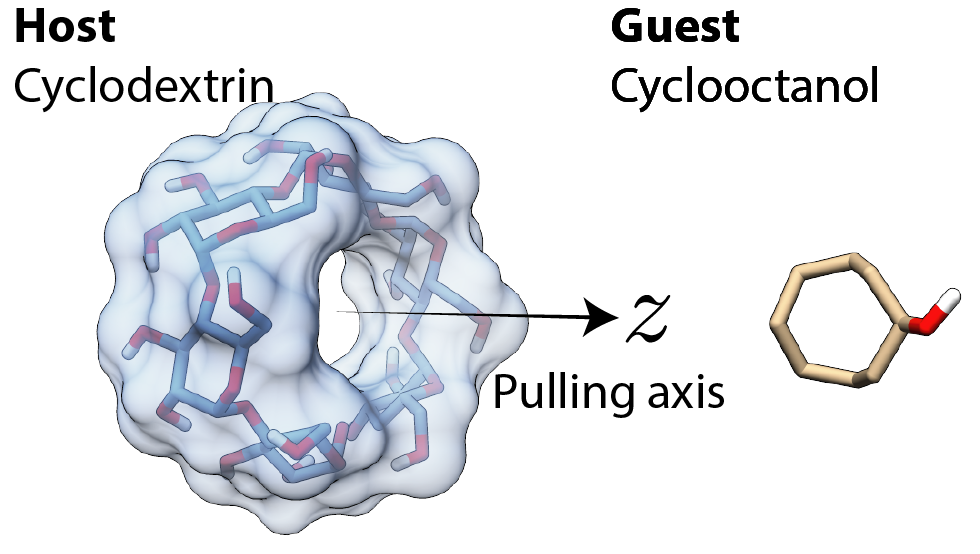
\includegraphics{content/images/APR-annotated.png}
\caption{An example host-guest system, \(\alpha\)-cyclodextrin with
cyclooctanol (unbound) showing the pulling coordinate along the \(z\)
axis.}
\label{fig:apr}
\end{wrapfloat}

Host-guest systems are noncovalent complexes between a cavity-like host
molecule and a small molecule guest. These systems retain many of the
same, strong functional group interactions of protein-ligand systems
while being computationally tractable and reaching convergence on a
shorter time scale. In the attach-pull-release (APR) method, the
reversible work of transferring the guest from the binding site to
solution, via a physical pathway, is computed using a series of umbrella
sampling windows (Figure \ref{fig:apr}). In the ``attach'' phase,
restraints are connected to the guest (and optionally, to the host for
better conformational sampling) through a parameter
\(\lambda \in [0, 1]\) that controls the strength of the restraints.
During the ``pull'' phase, the equilibrium length of a distance
restraint joining the guest and host is increased until the guest is no
longer interacting with the host molecule. The ``release'' phase
reverses the work of attaching the restraints and also corrects the
concentration of the guest molecule to standard state. Simulating each
window and integrating over the partial derivative of the restraint
energy with respect to the restraint target, we can generate a potential
of mean force along the pulling coordinate that is used to compute the
binding free energy at standard state, \(\Delta G^\circ\).

\hypertarget{incorporate-host-guest-binding-data-into-force-field-development}{%
\subsubsection{Incorporate host-guest binding data into force field
development}\label{incorporate-host-guest-binding-data-into-force-field-development}}

APR has consistently been ranked among the most accurate methods for
predicting binding thermodynamics in blind
challenges\textsuperscript{\protect\hyperlink{ref-BGsUYQln}{1},\protect\DIFdelbegin %DIFDELCMD < \hyperlink{ref-GA1AFcUw}{46}%%%
\DIFdelend \DIFaddbegin \hyperlink{ref-GA1AFcUw}{54}\DIFaddend }.
I will independently continue the development of APR, through its Python
interface, pAPRika, and transform it into a generalized tool that is
capable of computing free energies along any physical pathway, using
either AMBER or OpenMM as simulation packages. The core functionality of
pAPRika is already being used by research groups across the country and
in at least one group in China. Extending pAPRika would allow the same
rigorous thermodynamic framework to be used in applications such as
protein-protein interactions, dimerization of small molecules, or
nucleotide flipping. As part of the development, I will also investigate
the accuracy of non-pathway, end-point methods, such as the direct
calculation of interaction
entropy\textsuperscript{\protect\DIFdelbegin %DIFDELCMD < \hyperlink{ref-gRfhPG7N}{47}%%%
\DIFdelend \DIFaddbegin \hyperlink{ref-gRfhPG7N}{55}\DIFaddend }.

Most established small molecule force fields (e.g., the general AMBER
force field, GAFF) have been tuned using pure liquid state data, such as
the average density, enthalpy of vaporization, or the self-diffusion
coefficient. Over the past decade, it has become clear that reproducing
those properties well does not guarantee binding thermodynamics at a
level acceptable for guiding experiments. The open force field group
(OpenFF) aims to develop new, collaborative force fields using open
access methods, open source software, and high-quality open data sets.
One central difference with the OpenFF group is the use of direct
chemical perception to apply force field parameters based on a molecular
graph instead of atom
types\textsuperscript{\protect\DIFdelbegin %DIFDELCMD < \hyperlink{ref-HlBr7NrU}{48}%%%
\DIFdelend \DIFaddbegin \hyperlink{ref-HlBr7NrU}{56}\DIFaddend }, and the
desire to avoid over-fitting parameters by making Monte Carlo moves in
parameter space to find the fewest number of parameters required to
describe a set of
chemistries\textsuperscript{\protect\DIFdelbegin %DIFDELCMD < \hyperlink{ref-13lTSBgHy}{49}%%%
\DIFdelend \DIFaddbegin \hyperlink{ref-13lTSBgHy}{57}\DIFaddend }. The
first prototype force field from this effort was release in June 2018,
called SMIRNOFF99Frosst v0.1, based on a predecessor of GAFF.
SMIRNOFF99Frosst is able to perform as well as GAFF, and in some cases,
alleviate conformational problems caused by GAFF's atom types, in only
335 parameter lines compared to the 6794 lines in GAFF version 2.1.
Beyond this initial release, multiple generations of SMIRNOFF99Frosst
are planned, incorporating new forms of Lennard-Jones interactions, the
addition of atom polarizabilities, and Bayesian estimates to quantify
systematic errors in the force field.


\begin{wrapfloat}{figure}{R}{3in}
\centering
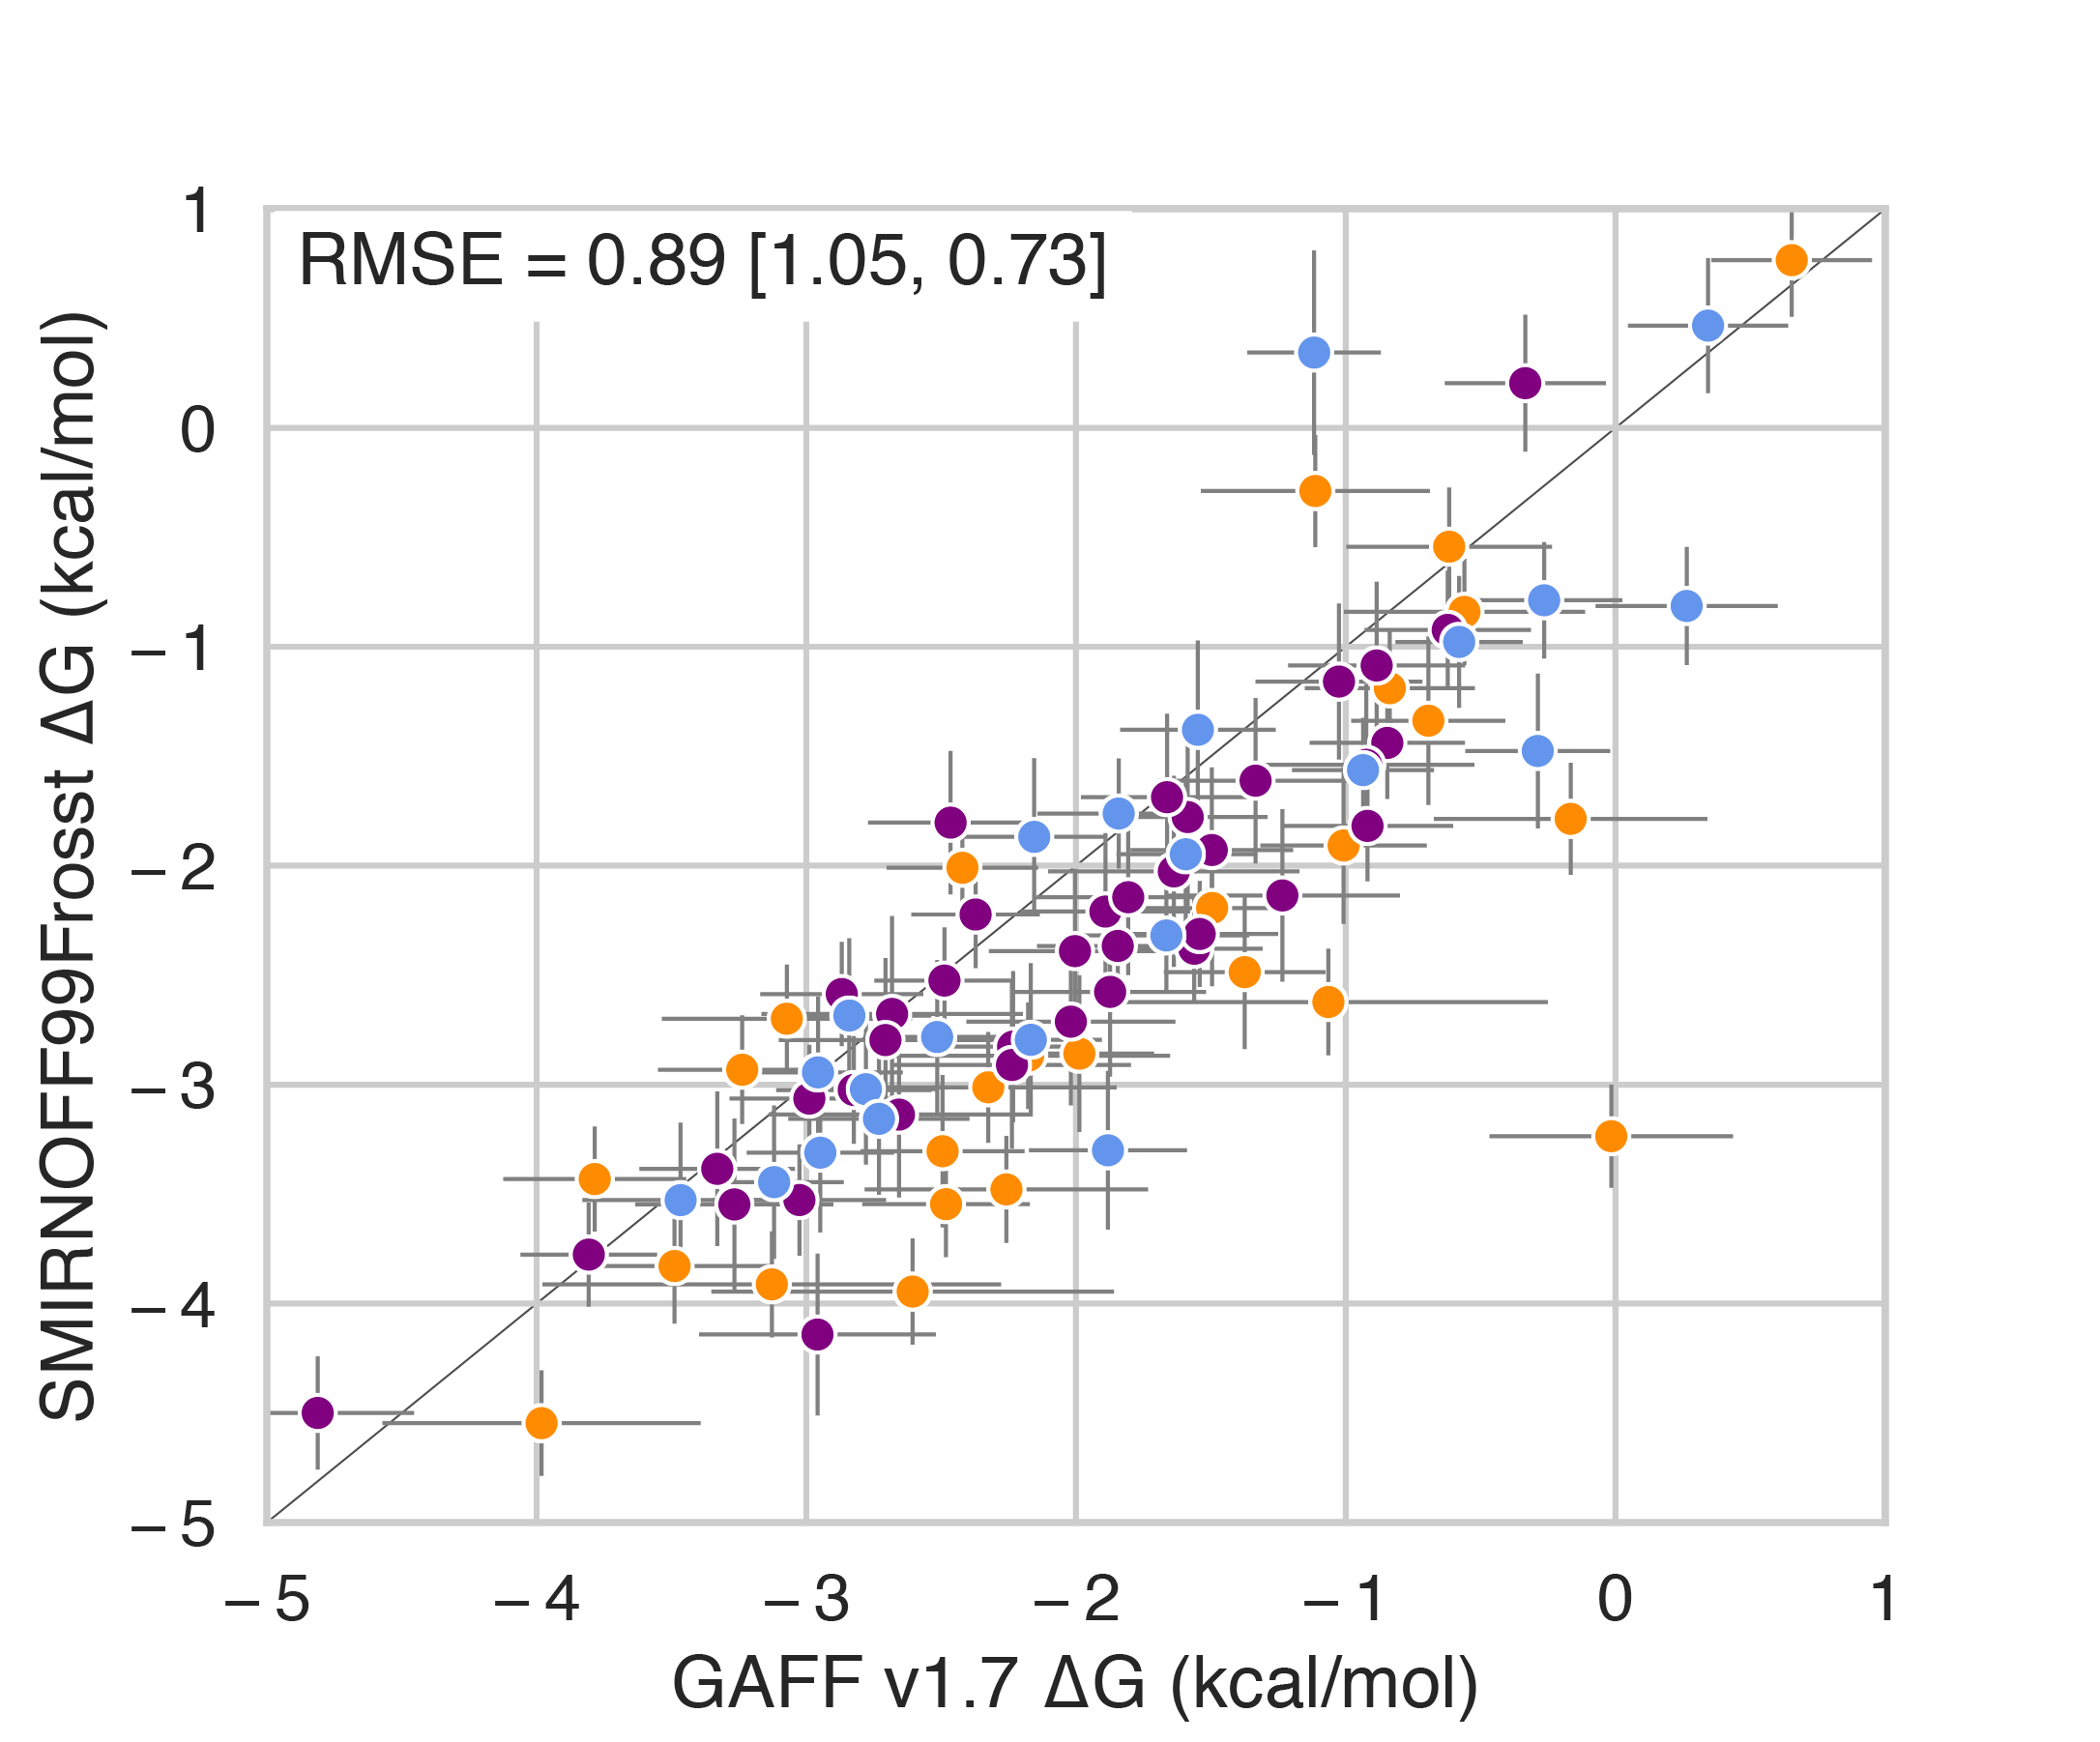
\includegraphics{content/images/SMIRNOFF-vs-GAFF-deltaG.png}
\caption{A comparison of binding free energies between SMIRNOFF99Frosst
and GAFF v1.7 for a series of cyclodextrin hosts and guests (unpublished
results). Points are colored according to guest functional group.}
\label{fig:smirnoff}
\end{wrapfloat}

As part of the OpenFF consortium, I will benchmark new iterations of
SMIRNOFF99Frosst using host-guest thermodynamics computed by pAPRika.
Figure \ref{fig:smirnoff} shows the very first comparison of
SMIRNOFF99Frosst v0.1 and GAFF v1.7 on host-guest systems. GAFF v1.7 is
known to overestimate binding affinities by \textgreater{}1
kcal/mol\textsuperscript{\protect\DIFdelbegin %DIFDELCMD < \hyperlink{ref-HVgz5rZq}{50}%%%
\DIFdelend \DIFaddbegin \hyperlink{ref-HVgz5rZq}{58}\DIFaddend }, and it
appears that SMIRNOFF99Frosst reduces this tendency. To begin, I will
use the ``\href{https://escholarship.org/uc/item/9p37m6bq}{benchmark
set}'' of Mobley et
al.\textsuperscript{\protect\DIFdelbegin %DIFDELCMD < \hyperlink{ref-12BD3oHp4}{51}%%%
\DIFdelend \DIFaddbegin \hyperlink{ref-12BD3oHp4}{59}\DIFaddend }. There,
experimental data are available for rigid curcurbituril and highly
flexible cyclodextrin hosts with a variety of drug-like guest molecules.
When available, I will also incorporate the binding data resulting from
selective derivatization of cyclodextrins designed to evaluate specific
functional group
interactions\textsuperscript{\protect\DIFdelbegin %DIFDELCMD < \hyperlink{ref-13gqBX78S}{52}%%%
\DIFdelend \DIFaddbegin \hyperlink{ref-13gqBX78S}{60}\DIFaddend }.
Enthalpies are poorly correlated with free energies, and thus, they
represent a nearly independent set of data to compare. I will match the
simulations to the experimental conditions, including host and guest
concentration, stoichiometry, ion concentration, and buffer conditions.
I will report metrics such as RMSE, R\textsuperscript{2}, Kendall's τ,
and the slope of the correlation between candidate parameter sets and
(a) a reference force field such as GAFF, CGenFF, or OPLS3 and (b) the
experimental thermodynamic data determined using ITC and NMR. The
results of my analysis will be reported through
\href{https://travis-ci.org/openforcefield/openforcefield?branch=master}{continuous
integration}, whereby each candidate update to the force field is
automatically tested through a clear and well-defined set of tests.

\hypertarget{integrate-automated-optimization-techniques-such-as-forcebalance-with-host-guest-binding-data}{%
\subsubsection{Integrate automated optimization techniques, such as
ForceBalance, with host-guest binding
data}\label{integrate-automated-optimization-techniques-such-as-forcebalance-with-host-guest-binding-data}}

As part of the open force field effort, we need to be able to rapidly
and efficiently optimize force field parameters given functional forms
and input data. ForceBalance is a tool, written by Dr.~Lee-Ping Wang,
that uses thermodynamic fluctuation formulas and reference data (e.g.,
\emph{ab initio} quantum mechanical calculations and experimentally
known molecular or bulk properties) to optimize an objective function,
such as the sum of squared differences between the calculated and
reference values ForceBalance has already been used to optimize water
models\textsuperscript{\protect\DIFdelbegin %DIFDELCMD < \hyperlink{ref-50lAQZra}{53}%%%
\DIFdelend \DIFaddbegin \hyperlink{ref-50lAQZra}{61}\DIFaddend } and protein
force fields\textsuperscript{\protect\DIFdelbegin %DIFDELCMD < \hyperlink{ref-1E3wArY0j}{54}%%%
\DIFdelend \DIFaddbegin \hyperlink{ref-1E3wArY0j}{62}\DIFaddend }. As
a member of the OpenFF consortium, Dr.~Wang has begun to add support for
the SMIRNOFF force field format. I will extend my collaboration with
Dr.~Wang to include pAPRika in the optimization loop of ForceBalance. I
have experience working with the analytic derivatives of the binding
free energy with respect to Lennard-Jones
parameters\textsuperscript{\protect\DIFdelbegin %DIFDELCMD < \hyperlink{ref-xRauI5mb}{55}%%%
\DIFdelend \DIFaddbegin \hyperlink{ref-xRauI5mb}{63}\DIFaddend }, and
using these derivatives to tune parameters was recently used by a
colleague to optimize the TIP3P water model for binding calculations by
post-processing existing MD trajectories for small parameter
perturbation\textsuperscript{\protect\DIFdelbegin %DIFDELCMD < \hyperlink{ref-NeqIQDLp}{56}%%%
\DIFdelend \DIFaddbegin \hyperlink{ref-NeqIQDLp}{64}\DIFaddend }.

A proximate goal is to create a method for passing a candidate set of
parameters from ForceBalance to pAPRika and for pAPRika to return an
estimate of the quality of the parameters in machine-readable format,
such as JSON or XML. The experimental data for ForceBalance will be
taken from the free and open
\href{https://www.nist.gov/mml/acmd/trc/thermoml}{ThermoML} database
curated by NIST. I will focus on including data that represent
intermolecular interactions, such as enthalpies of mixing and partition
coefficients, that will broaden the data used for force field
development beyond single species properties. Host-guest calculations
are computationally expensive, sometimes requiring \textgreater{}1
GPU-day to reach the desired level of convergence, and this has the
potential to significantly slow down ForceBalance. I will add the
ability to automatically allocate resources in the APR calculation, by
calculating the return on investment (ROI) in each window. The ROI is
the partial derivative of the overall standard error of the mean binding
affinity with respect to the number of frames in window \(i\),
\(\partial G^\circ_\text{SEM} / \partial N^i_\text{frames}\) . This will
allow us to simulate each window long enough such that the overall
estimate of the binding free energy reaches below a certain threshold.

Together, these methodological improvements will help create a
transparent and robust set of metrics to evaluate the performance of
candidate force fields on an equal footing. By incorporating host-guest
binding data, the degeneracy in parameter space will be broken, avoiding
force fields that agree excellently with experiment for liquid
properties and yet agree poorly on binding. I believe the ideas in this
aim could be turned into an NIH proposal by demonstrating the need to
systematically evaluate force field accuracy for protein-ligand binding,
perhaps the most important application of this work for human health.

\DIFaddbegin \hypertarget{building-better-force-fields-for-drug-discovery-using-open-data-and-automated-optimization-1}{%
\subsection{Building better force fields for drug discovery using open
data and automated
optimization}\label{building-better-force-fields-for-drug-discovery-using-open-data-and-automated-optimization-1}}

\DIFadd{Designing ligands that bind their target with high affinity and
specificity is the principal objective of small-molecule drug discovery,
yet hit-to-lead and lead-optimization can take upwards of three years
owing to the fact it is often necessary to synthesize hundreds or
thousands of new compounds. In short, drug discovery is very expensive
and often fails. In recent years, the pharmaceutical industry has begun
to use absolute and relative binding free energy calculations to help
narrow the number of compounds that must be
synthesized\textsuperscript{\protect\hyperlink{ref-1FiDpP1LR}{48},\protect\hyperlink{ref-1BwXH3GFO}{49}}.
In particular, the advent of computational calorimetry has enabled
quantitative and high-precision comparisons of binding free energies,
enthalpies, and entropies (by subtraction) with experimental values
determined by isothermal titration calorimetry or
NMR\textsuperscript{\protect\hyperlink{ref-1935a9V0d}{50}}. The root
mean squared error (RMSE) associated with such calculations is in the
range of 1-4
kcal/mol\textsuperscript{\protect\hyperlink{ref-LWd10vQy}{51}}, yet even
a modest improvement of the prediction accuracy of \textasciitilde{}1
kcal/mol would lead to a substantial decrease in the number of compounds
that must be manually screened by nearly an order of
magnitude\textsuperscript{\protect\hyperlink{ref-fC0t6Cy1}{52}}.
Although it has been suggested by some that changes in the force field
functional form are required, it is clear that there is ample room to
improve the accuracy of existing parameters through careful
analysis\textsuperscript{\protect\hyperlink{ref-LOjcxYqt}{53}}. The
first goal of this aim is to create better tools to guide early-stage
drug discovery by reducing the number of compounds that must be
synthesized to find a promising hit that can be carried over into
clinical trials.
}


\begin{wrapfloat}{figure}{L}{3in}
\centering
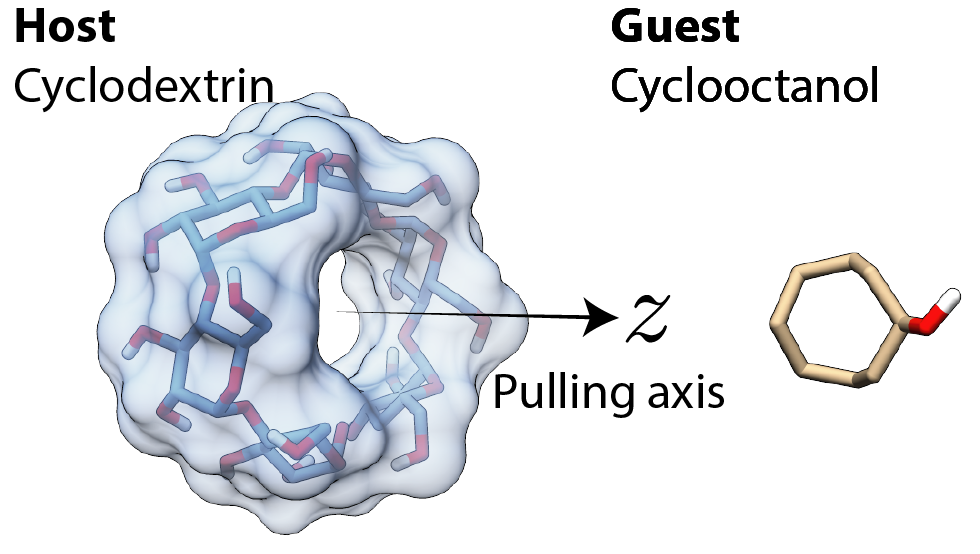
\includegraphics{content/images/APR-annotated.png}
\caption{\DIFadd{An example host-guest system, \(\alpha\)-cyclodextrin with
cyclooctanol (unbound) showing the pulling coordinate along the \(z\)
axis.}}
\label{fig:apr}
\end{wrapfloat}

\DIFadd{Host-guest systems are noncovalent complexes between a cavity-like host
molecule and a small molecule guest. These systems retain many of the
same, strong functional group interactions of protein-ligand systems
while being computationally tractable and reaching convergence on a
shorter time scale. In the attach-pull-release (APR) method, the
reversible work of transferring the guest from the binding site to
solution, via a physical pathway, is computed using a series of umbrella
sampling windows (Figure \ref{fig:apr}). In the ``attach'' phase,
restraints are connected to the guest (and optionally, to the host for
better conformational sampling) through a parameter
\(\lambda \in [0, 1]\) that controls the strength of the restraints.
During the ``pull'' phase, the equilibrium length of a distance
restraint joining the guest and host is increased until the guest is no
longer interacting with the host molecule. The ``release'' phase
reverses the work of attaching the restraints and also corrects the
concentration of the guest molecule to standard state. Simulating each
window and integrating over the partial derivative of the restraint
energy with respect to the restraint target, we can generate a potential
of mean force along the pulling coordinate that is used to compute the
binding free energy at standard state, \(\Delta G^\circ\).
}

\hypertarget{incorporate-host-guest-binding-data-into-force-field-development-1}{%
\subsubsection{Incorporate host-guest binding data into force field
development}\label{incorporate-host-guest-binding-data-into-force-field-development-1}}

\DIFadd{APR has consistently been ranked among the most accurate methods for
predicting binding thermodynamics in blind
challenges\textsuperscript{\protect\hyperlink{ref-BGsUYQln}{1},\protect\hyperlink{ref-GA1AFcUw}{54}}.
I will independently continue the development of APR, through its Python
interface, pAPRika, and transform it into a generalized tool that is
capable of computing free energies along any physical pathway, using
either AMBER or OpenMM as simulation packages. The core functionality of
pAPRika is already being used by research groups across the country and
in at least one group in China. Extending pAPRika would allow the same
rigorous thermodynamic framework to be used in applications such as
protein-protein interactions, dimerization of small molecules, or
nucleotide flipping. As part of the development, I will also investigate
the accuracy of non-pathway, end-point methods, such as the direct
calculation of interaction
entropy\textsuperscript{\protect\hyperlink{ref-gRfhPG7N}{55}}.
}

\DIFadd{Most established small molecule force fields (e.g., the general AMBER
force field, GAFF) have been tuned using pure liquid state data, such as
the average density, enthalpy of vaporization, or the self-diffusion
coefficient. Over the past decade, it has become clear that reproducing
those properties well does not guarantee binding thermodynamics at a
level acceptable for guiding experiments. The open force field group
(OpenFF) aims to develop new, collaborative force fields using open
access methods, open source software, and high-quality open data sets.
One central difference with the OpenFF group is the use of direct
chemical perception to apply force field parameters based on a molecular
graph instead of atom
types\textsuperscript{\protect\hyperlink{ref-HlBr7NrU}{56}}, and the
desire to avoid over-fitting parameters by making Monte Carlo moves in
parameter space to find the fewest number of parameters required to
describe a set of
chemistries\textsuperscript{\protect\hyperlink{ref-13lTSBgHy}{57}}. The
first prototype force field from this effort was release in June 2018,
called SMIRNOFF99Frosst v0.1, based on a predecessor of GAFF.
SMIRNOFF99Frosst is able to perform as well as GAFF, and in some cases,
alleviate conformational problems caused by GAFF's atom types, in only
335 parameter lines compared to the 6794 lines in GAFF version 2.1.
Beyond this initial release, multiple generations of SMIRNOFF99Frosst
are planned, incorporating new forms of Lennard-Jones interactions, the
addition of atom polarizabilities, and Bayesian estimates to quantify
systematic errors in the force field.
}


\begin{wrapfloat}{figure}{R}{3in}
\centering
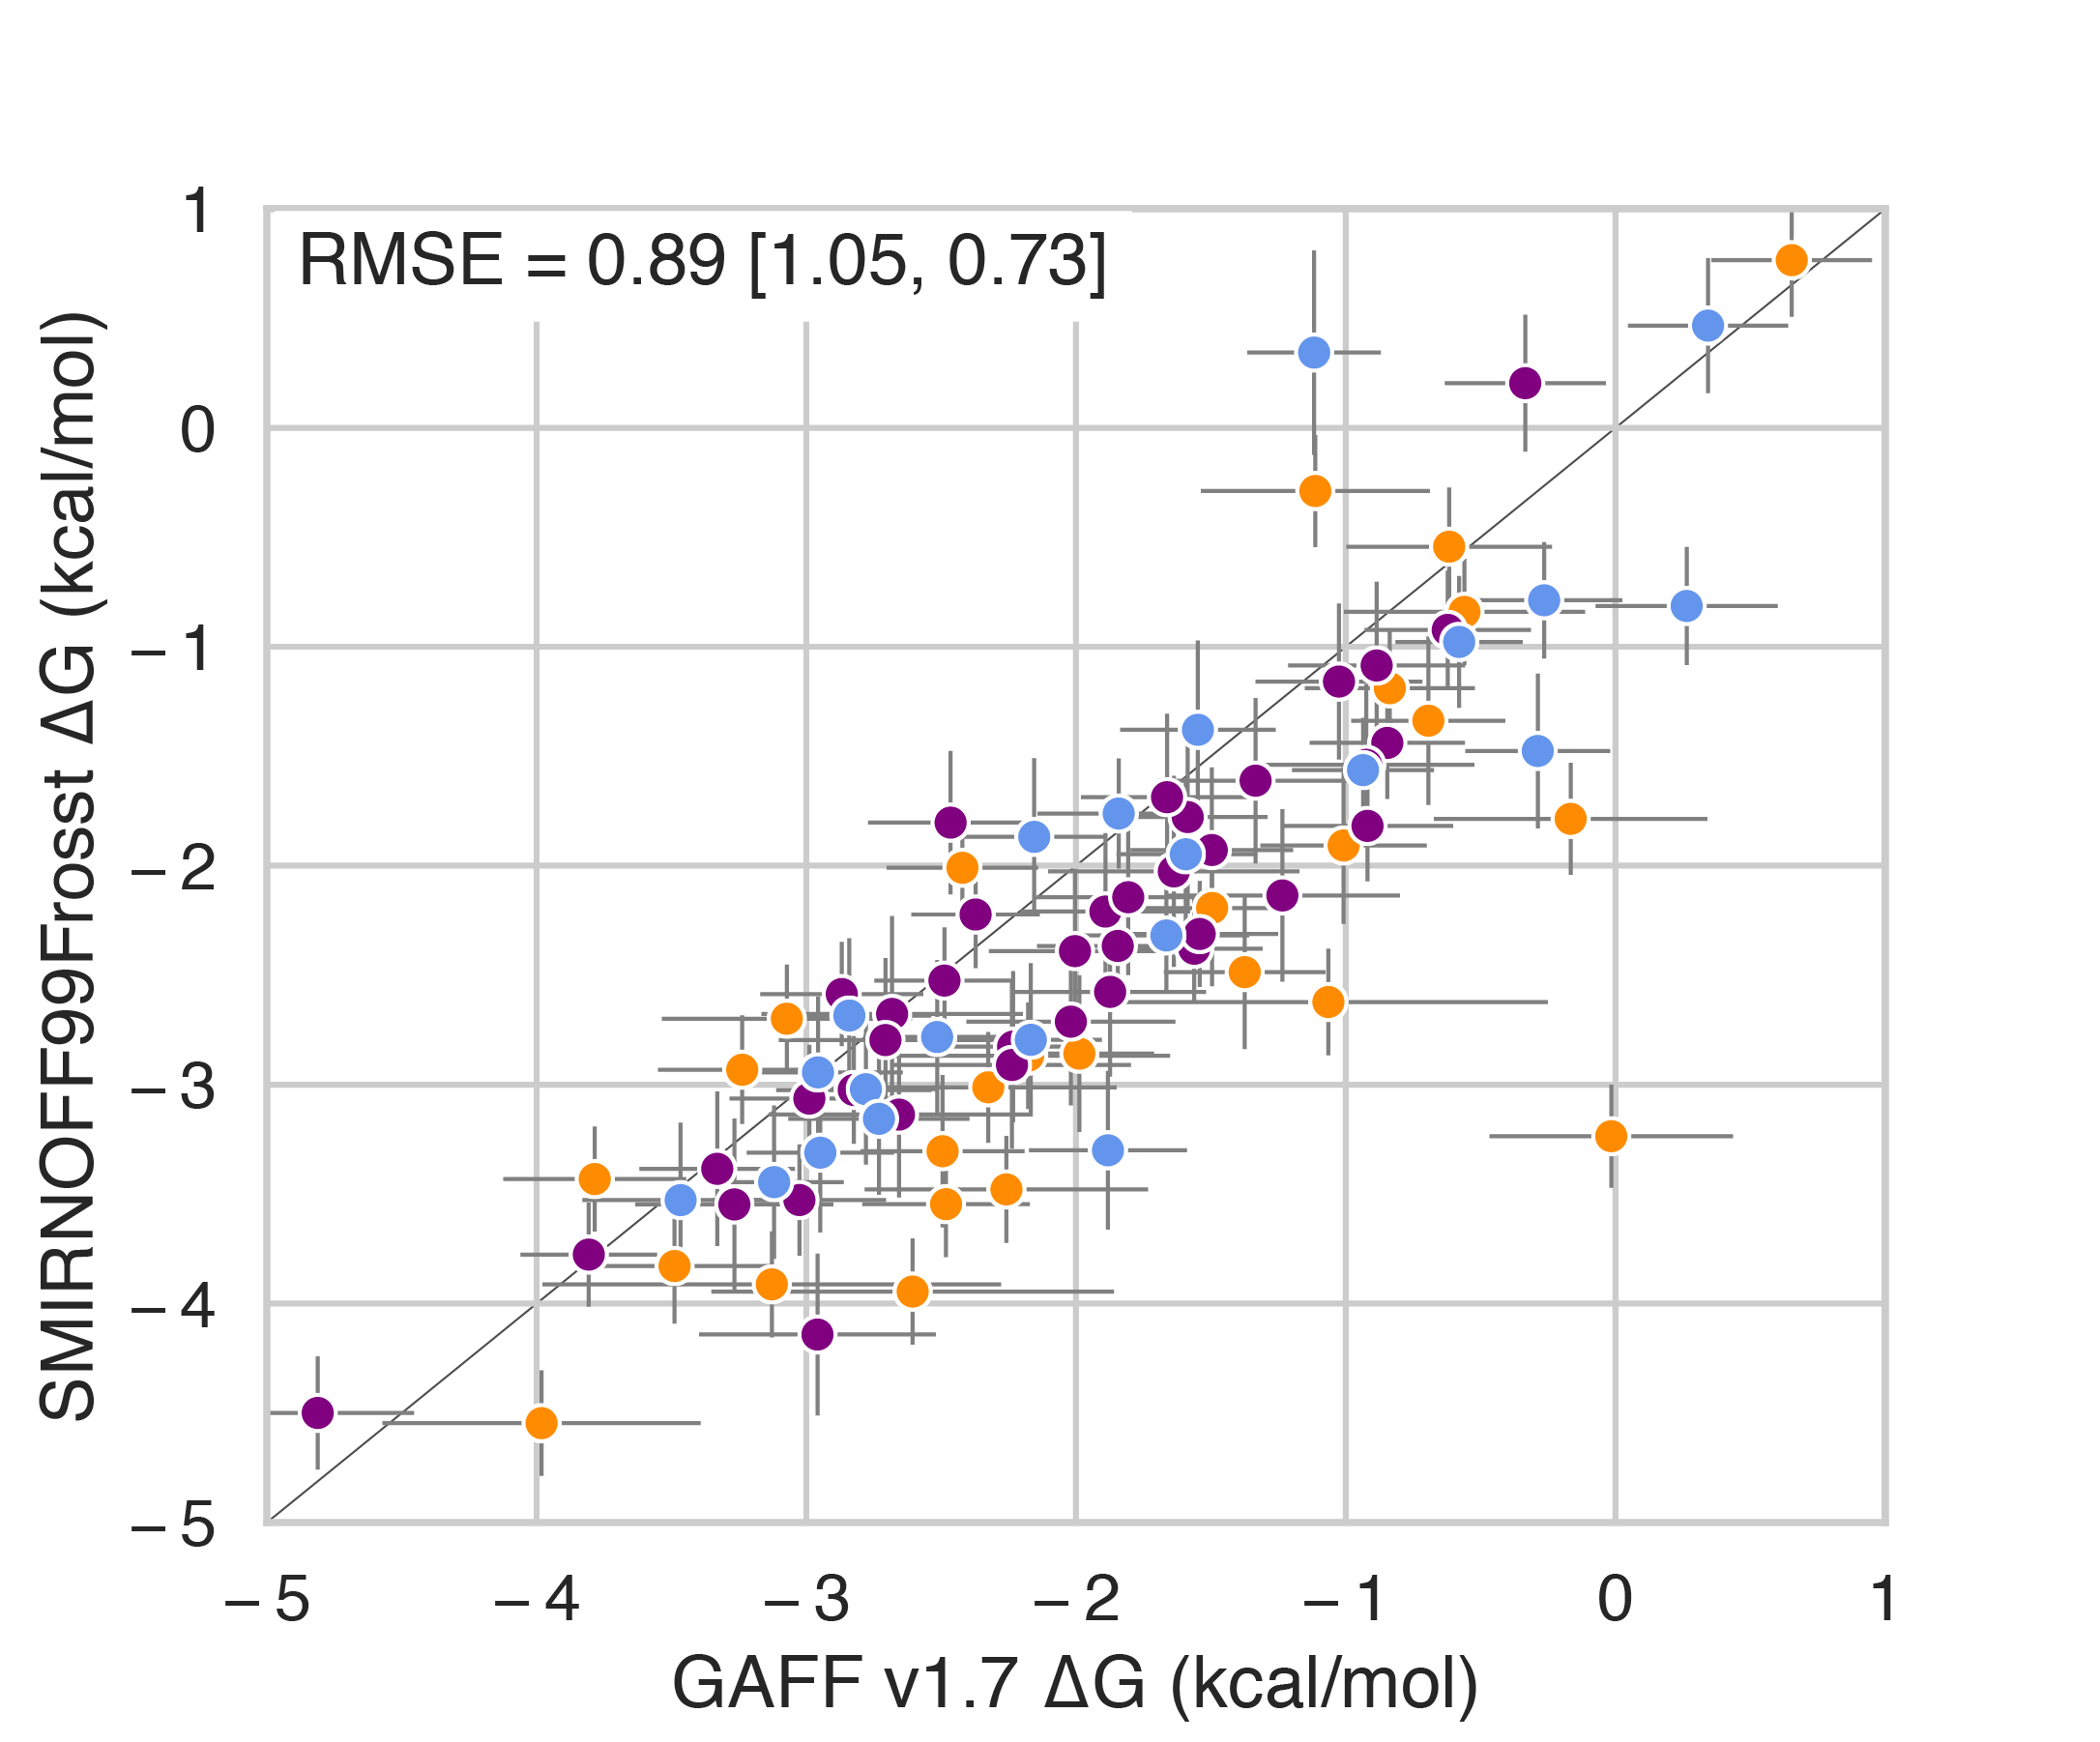
\includegraphics{content/images/SMIRNOFF-vs-GAFF-deltaG.png}
\caption{\DIFadd{A comparison of binding free energies between SMIRNOFF99Frosst
and GAFF v1.7 for a series of cyclodextrin hosts and guests (unpublished
results). Points are colored according to guest functional group.}}
\label{fig:smirnoff}
\end{wrapfloat}

\DIFadd{As part of the OpenFF consortium, I will benchmark new iterations of
SMIRNOFF99Frosst using host-guest thermodynamics computed by pAPRika.
Figure \ref{fig:smirnoff} shows the very first comparison of
SMIRNOFF99Frosst v0.1 and GAFF v1.7 on host-guest systems. GAFF v1.7 is
known to overestimate binding affinities by \textgreater{}1
kcal/mol\textsuperscript{\protect\hyperlink{ref-HVgz5rZq}{58}}, and it
appears that SMIRNOFF99Frosst reduces this tendency. To begin, I will
use the ``}\href{https://escholarship.org/uc/item/9p37m6bq}{benchmark
set}\DIFadd{'' of Mobley et
al.\textsuperscript{\protect\hyperlink{ref-12BD3oHp4}{59}}. There,
experimental data are available for rigid curcurbituril and highly
flexible cyclodextrin hosts with a variety of drug-like guest molecules.
When available, I will also incorporate the binding data resulting from
selective derivatization of cyclodextrins designed to evaluate specific
functional group
interactions\textsuperscript{\protect\hyperlink{ref-13gqBX78S}{60}}.
Enthalpies are poorly correlated with free energies, and thus, they
represent a nearly independent set of data to compare. I will match the
simulations to the experimental conditions, including host and guest
concentration, stoichiometry, ion concentration, and buffer conditions.
I will report metrics such as RMSE, R\textsuperscript{2}, Kendall's τ,
and the slope of the correlation between candidate parameter sets and
(a) a reference force field such as GAFF, CGenFF, or OPLS3 and (b) the
experimental thermodynamic data determined using ITC and NMR. The
results of my analysis will be reported through
}\href{https://travis-ci.org/openforcefield/openforcefield?branch=master}{continuous
integration}\DIFadd{, whereby each candidate update to the force field is
automatically tested through a clear and well-defined set of tests.
}

\hypertarget{integrate-automated-optimization-techniques-such-as-forcebalance-with-host-guest-binding-data-1}{%
\subsubsection{Integrate automated optimization techniques, such as
ForceBalance, with host-guest binding
data}\label{integrate-automated-optimization-techniques-such-as-forcebalance-with-host-guest-binding-data-1}}

\DIFadd{As part of the open force field effort, we need to be able to rapidly
and efficiently optimize force field parameters given functional forms
and input data. ForceBalance is a tool, written by Dr.~Lee-Ping Wang,
that uses thermodynamic fluctuation formulas and reference data (e.g.,
}\emph{\DIFadd{ab initio}} \DIFadd{quantum mechanical calculations and experimentally
known molecular or bulk properties) to optimize an objective function,
such as the sum of squared differences between the calculated and
reference values ForceBalance has already been used to optimize water
models\textsuperscript{\protect\hyperlink{ref-50lAQZra}{61}} and protein
force fields\textsuperscript{\protect\hyperlink{ref-1E3wArY0j}{62}}. As
a member of the OpenFF consortium, Dr.~Wang has begun to add support for
the SMIRNOFF force field format. I will extend my collaboration with
Dr.~Wang to include pAPRika in the optimization loop of ForceBalance. I
have experience working with the analytic derivatives of the binding
free energy with respect to Lennard-Jones
parameters\textsuperscript{\protect\hyperlink{ref-xRauI5mb}{63}}, and
using these derivatives to tune parameters was recently used by a
colleague to optimize the TIP3P water model for binding calculations by
post-processing existing MD trajectories for small parameter
perturbation\textsuperscript{\protect\hyperlink{ref-NeqIQDLp}{64}}.
}

\DIFadd{A proximate goal is to create a method for passing a candidate set of
parameters from ForceBalance to pAPRika and for pAPRika to return an
estimate of the quality of the parameters in machine-readable format,
such as JSON or XML. The experimental data for ForceBalance will be
taken from the free and open
}\href{https://www.nist.gov/mml/acmd/trc/thermoml}{ThermoML} \DIFadd{database
curated by NIST. I will focus on including data that represent
intermolecular interactions, such as enthalpies of mixing and partition
coefficients, that will broaden the data used for force field
development beyond single species properties. Host-guest calculations
are computationally expensive, sometimes requiring \textgreater{}1
GPU-day to reach the desired level of convergence, and this has the
potential to significantly slow down ForceBalance. I will add the
ability to automatically allocate resources in the APR calculation, by
calculating the return on investment (ROI) in each window. The ROI is
the partial derivative of the overall standard error of the mean binding
affinity with respect to the number of frames in window \(i\),
\(\partial G^\circ_\text{SEM} / \partial N^i_\text{frames}\) . This will
allow us to simulate each window long enough such that the overall
estimate of the binding free energy reaches below a certain threshold.
}

\DIFadd{Together, these methodological improvements will help create a
transparent and robust set of metrics to evaluate the performance of
candidate force fields on an equal footing. By incorporating host-guest
binding data, the degeneracy in parameter space will be broken, avoiding
force fields that agree excellently with experiment for liquid
properties and yet agree poorly on binding. I believe the ideas in this
aim could be turned into an NIH proposal by demonstrating the need to
systematically evaluate force field accuracy for protein-ligand binding,
perhaps the most important application of this work for human health.
}

\DIFaddend \pagebreak
\setlength{\parskip}{0.1mm}

\hypertarget{references}{%
\section*{References}\label{references}}
\addcontentsline{toc}{section}{References}

\setstretch{1}

\DIFaddbegin \pagebreak
\setlength{\parskip}{0.1mm}

\hypertarget{references-1}{%
\section*{References}\label{references-1}}
\addcontentsline{toc}{section}{\DIFadd{References}}

\setstretch{1}

\DIFaddend \hypertarget{refs}{}
\leavevmode\hypertarget{ref-BGsUYQln}{}%
(1) Yin, J.; Henriksen, N. M.; Slochower, D. R.; Shirts, M. R.; Chiu, M.
W.; Mobley, D. L.; Gilson, M. K. Overview of the SAMPL5 Host--Guest
Challenge: Are We Doing Better? \emph{J Comput Aided Mol Des}
\textbf{2016}, \emph{31} (1), 1--19.

\leavevmode\hypertarget{ref-uzHaEv9Z}{}%
(2) Yin, J.; Henriksen, N. M.; Slochower, D. R.; Gilson, M. K. The
SAMPL5 Host--Guest Challenge: Computing Binding Free Energies
and~Enthalpies from Explicit Solvent Simulations by the
Attach-Pull-Release (APR) Method. \emph{J Comput Aided Mol Des}
\textbf{2016}, \emph{31} (1), 133--145.

\leavevmode\hypertarget{ref-1BfYw0gk2}{}%
(3) Slochower, D. R.; Gilson, M. K. Motor-Like Properties of Nonmotor
Enzymes. \emph{Biophysical Journal} \textbf{2018}, \emph{114} (9),
2174--2179.

\leavevmode\hypertarget{ref-1G0A01ZNq}{}%
(4) Slochower, D. R.; Huwe, P. J.; Radhakrishnan, R.; Janmey, P. A.
Quantum and All-Atom Molecular Dynamics Simulations of Protonation and
Divalent Ion Binding to Phosphatidylinositol 4,5-Bisphosphate (PIP2).
\emph{J. Phys. Chem. B} \textbf{2013}, \emph{117} (28), 8322--8329.

\leavevmode\hypertarget{ref-SdO7fVnR}{}%
(5) Slochower, D. R.; Wang, Y.-H.; Tourdot, R. W.; Radhakrishnan, R.;
Janmey, P. A. Counterion-Mediated Pattern Formation in Membranes
Containing Anionic Lipids. \emph{Advances in Colloid and Interface
Science} \textbf{2014}, \emph{208}, 177--188.

\leavevmode\hypertarget{ref-Ag1rh6TA}{}%
(6) Wang, Y.-H.; Slochower, D. R.; Janmey, P. A. Counterion-Mediated
Cluster Formation by Polyphosphoinositides. \emph{Chemistry and Physics
of Lipids} \textbf{2014}, \emph{182}, 38--51.

\leavevmode\hypertarget{ref-1E1rz4J4o}{}%
(7) Slochower, D. R.; Wang, Y.-H.; Radhakrishnan, R.; Janmey, P. A.
Physical Chemistry and Membrane Properties of Two Phosphatidylinositol
Bisphosphate Isomers. \emph{Phys. Chem. Chem. Phys.} \textbf{2015},
\emph{17} (19), 12608--12615.

\leavevmode\hypertarget{ref-1AHXI1BtY}{}%
(8) Slochower, D. R.; Wang, Y.-H.; Radhakrishnan, R.; Janmey, P. A.
Lipid Membrane Shape Evolution and the Actin Cytoskeleton. In
\emph{Handbook of Lipid Membranes, Molecular and Materials aspects};
Safinya, C., Rädler, J., Series Eds.; Taylor \& Francis Publishers,
2018.

\leavevmode\hypertarget{ref-GGlssBvj}{}%
(9) Di Paolo, G.; De Camilli, P. Phosphoinositides in Cell Regulation
and Membrane Dynamics. \emph{Nature} \textbf{2006}, \emph{443} (7112),
651--657.

\leavevmode\hypertarget{ref-8Xw2kuUO}{}%
(10) Faiderbe, S.; Chagnaud, J.-L.; Geffard, M. Anti-Phosphoinositide
Auto-Antibodies in Sera of Cancer Patients: Isotypic and Immunochemical
Characterization. \emph{Cancer Letters} \textbf{1992}, \emph{66} (1),
35--41.

\leavevmode\hypertarget{ref-12CAxA8dE}{}%
(11) Lin, W.; Leung, L. W.; Bae, Y. S.; Bittman, R.; Arthur, G. Effects
of a Water-Soluble Antitumor Ether Phosphonoinositide, d-Myo-Inositol
4-(Hexadecyloxy)-3(S)-Methoxybutanephosphonate (C4-Pi), on Inositol
Lipid Metabolism in Breast Epithelial Cancer Cell Lines.
\emph{Biochemical Pharmacology} \textbf{1999}, \emph{57} (10),
1153--1158.

\leavevmode\hypertarget{ref-l2gqdgv}{}%
(12) Katso, R.; Okkenhaug, K.; Ahmadi, K.; White, S.; Timms, J.;
Waterfield, M. D. Cellular Function of Phosphoinositide 3-Kinases:
Implications for Development, Immunity, Homeostasis, and Cancer.
\emph{Annu. Rev. Cell Dev. Biol.} \textbf{2001}, \emph{17} (1),
615--675.

\leavevmode\hypertarget{ref-izLqFTEH}{}%
(13) Engelman, J. A. The Role of Phosphoinositide 3-Kinase Pathway
Inhibitors in the Treatment of Lung Cancer. \emph{Clinical Cancer
Research} \textbf{2007}, \emph{13} (15), 4637s--4640s.

\leavevmode\hypertarget{ref-1HRoQaadQ}{}%
(14) Miled, N.; Yan, Y.; Hon, W.-C.; Perisic, O.; Zvelebil, M.; Inbar,
Y.; Schneidman-Duhovny, D.; Wolfson, H. J.; Backer, J. M.; Williams, R.
L. Mechanism of Two Classes of Cancer Mutations in the Phosphoinositide
3-Kinase Catalytic Subunit. \emph{Science} \textbf{2007}, \emph{317}
(5835), 239--242.

\leavevmode\hypertarget{ref-1DCzqvykg}{}%
(15) Bunney, T. D.; Katan, M. Phosphoinositide Signalling in Cancer:
Beyond PI3K and PTEN. \emph{Nat Rev Cancer} \textbf{2010}, \emph{10}
(5), 342--352.

\leavevmode\hypertarget{ref-uyKE7bWV}{}%
(16) Lemmon, M. A. Membrane Recognition by Phospholipid-Binding Domains.
\emph{Nat Rev Mol Cell Biol} \textbf{2008}, \emph{9} (2), 99--111.

\leavevmode\hypertarget{ref-3EmJ4esY}{}%
(17) McLaughlin, S.; Wang, J.; Gambhir, A.; Murray, D. PIP2 and
Proteins: Interactions, Organization, and Information Flow. \emph{Annu.
Rev. Biophys. Biomol. Struct.} \textbf{2002}, \emph{31} (1), 151--175.

\leavevmode\hypertarget{ref-5PUA7pLD}{}%
(18) Bradley, R.; Radhakrishnan, R. Curvature-Undulation Coupling as a
Basis for Curvature Sensing and Generation in Bilayer Membranes.
\emph{Biophysical Journal} \textbf{2017}, \emph{112} (3), 220a--221a.

\leavevmode\hypertarget{ref-8pFCG7HG}{}%
(19) Kooijman, E. E.; King, K. E.; Gangoda, M.; Gericke, A. Ionization
Properties of Phosphatidylinositol Polyphosphates in Mixed Model
Membranes. \emph{Biochemistry} \textbf{2009}, \emph{48} (40),
9360--9371.

\leavevmode\hypertarget{ref-U2YHSNKE}{}%
(20) van den Bogaart, G.; Meyenberg, K.; Risselada, H. J.; Amin, H.;
Willig, K. I.; Hubrich, B. E.; Dier, M.; Hell, S. W.; Grubmüller, H.;
Diederichsen, U.; et al. Membrane Protein Sequestering by Ionic
Protein--Lipid Interactions. \emph{Nature} \textbf{2011}, \emph{479}
(7374), 552--555.

\leavevmode\hypertarget{ref-Gw4f4Ayu}{}%
(21) Honigmann, A.; van den Bogaart, G.; Iraheta, E.; Risselada, H. J.;
Milovanovic, D.; Mueller, V.; Müllar, S.; Diederichsen, U.; Fasshauer,
D.; Grubmüller, H.; et al. Phosphatidylinositol 4,5-Bisphosphate
Clusters Act as Molecular Beacons for Vesicle Recruitment. \emph{Nat
Struct Mol Biol} \textbf{2013}, \emph{20} (6), 679--686.

\leavevmode\hypertarget{ref-rvpDeSHJ}{}%
(22) Wang, J.; Richards, D. A. Segregation of PIP2 and PIP3 into
Distinct Nanoscale Regions Within the Plasma Membrane. \emph{Biology
Open} \textbf{2012}, \emph{1} (9), 857--862.

\leavevmode\hypertarget{ref-LhOwGz4k}{}%
(23) Wang, Y.-H.; Collins, A.; Guo, L.; Smith-Dupont, K. B.; Gai, F.;
Svitkina, T.; Janmey, P. A. Divalent Cation-Induced Cluster Formation by
Polyphosphoinositides in Model Membranes. \emph{J. Am. Chem. Soc.}
\textbf{2012}, \emph{134} (7), 3387--3395.

\leavevmode\hypertarget{ref-ior8wlwH}{}%
(24) Wen, Y.; Vogt, V. M.; Feigenson, G. W. Multivalent Cation-Bridged
PI(4,5)P 2 Clusters Form at Very Low Concentrations. \emph{Biophysical
Journal} \textbf{2018}, \emph{114} (11), 2630--2639.

\leavevmode\hypertarget{ref-JWXdIfNt}{}%
(25) Levental, I.; Christian, D. A.; Wang, Y.-H.; Madara, J. J.;
Discher, D. E.; Janmey, P. A. Calcium-Dependent Lateral Organization in
Phosphatidylinositol 4,5-Bisphosphate (PIP2)- and Cholesterol-Containing
Monolayers. \emph{Biochemistry} \textbf{2009}, \emph{48} (34),
8241--8248.

\leavevmode\hypertarget{ref-14RTQvTQS}{}%
(26) BioPhysCode \url{https://github.com/biophyscode}.

\leavevmode\hypertarget{ref-aHkuGDrS}{}%
(27) BioPhysCode Portal \url{https://biophyscode.github.io/}.

\leavevmode\DIFdelbegin %DIFDELCMD < \hypertarget{ref-18PGyWtWV}{}%%%
\DIFdelend \DIFaddbegin \hypertarget{ref-GGtK2c0N}{}\DIFaddend %
(28) \DIFaddbegin \DIFadd{Gidwani, A.; Holowka, D.; Baird, B. Fluorescence Anisotropy
Measurements of Lipid Order in Plasma Membranes and Lipid Rafts from
RBL-2H3 Mast Cells†. }\emph{\DIFadd{Biochemistry}} \textbf{\DIFadd{2001}}\DIFadd{, }\emph{\DIFadd{40}} \DIFadd{(41),
12422--12429.
}

\leavevmode\hypertarget{ref-1Eg1Hzju1}{}%DIF > 
\DIFadd{(29) Swamy, M. J.; Ciani, L.; Ge, M.; Smith, A. K.; Holowka, D.; Baird,
B.; Freed, J. H. Coexisting Domains in the Plasma Membranes of Live
Cells Characterized by Spin-Label ESR Spectroscopy. }\emph{\DIFadd{Biophysical
Journal}} \textbf{\DIFadd{2006}}\DIFadd{, }\emph{\DIFadd{90}} \DIFadd{(12), 4452--4465.
}

\leavevmode\hypertarget{ref-oBaB5Z87}{}%DIF > 
\DIFadd{(30) Levental, I.; Byfield, F.; Chowdhury, P.; Gai, F.; Baumgart, T.;
Janmey, P. Cholesterol-Dependent Phase Separation in Cell-Derived Giant
Plasma-Membrane Vesicles. }\emph{\DIFadd{Biochem. J.}} \textbf{\DIFadd{2009}}\DIFadd{, }\emph{\DIFadd{424}}
\DIFadd{(2), 163--167.
}

\leavevmode\hypertarget{ref-BzP79Vj9}{}%DIF > 
\DIFadd{(31) Sengupta, P.; Holowka, D.; Baird, B. Fluorescence Resonance Energy
Transfer Between Lipid Probes Detects Nanoscopic Heterogeneity in the
Plasma Membrane of Live Cells. }\emph{\DIFadd{Biophysical Journal}} \textbf{\DIFadd{2007}}\DIFadd{,
}\emph{\DIFadd{92}} \DIFadd{(10), 3564--3574.
}

\leavevmode\hypertarget{ref-aiu6Tmil}{}%DIF > 
\DIFadd{(32) Baumgart, T.; Hammond, A. T.; Sengupta, P.; Hess, S. T.; Holowka,
D. A.; Baird, B. A.; Webb, W. W. Large-Scale Fluid/Fluid Phase
Separation of Proteins and Lipids in Giant Plasma Membrane Vesicles.
}\emph{\DIFadd{Proceedings of the National Academy of Sciences}} \textbf{\DIFadd{2007}}\DIFadd{,
}\emph{\DIFadd{104}} \DIFadd{(9), 3165--3170.
}

\leavevmode\hypertarget{ref-10CqL9t0a}{}%DIF > 
\DIFadd{(33) Ellenbroek, W.; Wang, Y.-H.; Christian, D.; Discher, D.; Janmey,
P.; Liu, A. Divalent Cation-Dependent Formation of Electrostatic PIP2
Clusters in Lipid Monolayers. }\emph{\DIFadd{Biophysical Journal}} \textbf{\DIFadd{2011}}\DIFadd{,
}\emph{\DIFadd{101}} \DIFadd{(9), 2178--2184.
}

\leavevmode\hypertarget{ref-XIltXoGI}{}%DIF > 
\DIFadd{(34) Heinrich, M.; Tian, A.; Esposito, C.; Baumgart, T. Dynamic Sorting
of Lipids and Proteins in Membrane Tubes with a Moving Phase Boundary.
}\emph{\DIFadd{Proceedings of the National Academy of Sciences}} \textbf{\DIFadd{2010}}\DIFadd{,
}\emph{\DIFadd{107}} \DIFadd{(16), 7208--7213.
}

\leavevmode\hypertarget{ref-2TfZ4zWV}{}%DIF > 
\DIFadd{(35) Raghunathan, K.; Kenworthy, A. K. Dynamic Pattern Generation in
Cell Membranes: Current Insights into Membrane Organization.
}\emph{\DIFadd{Biochimica et Biophysica Acta (BBA) - Biomembranes}} \textbf{\DIFadd{2018}}\DIFadd{,
}\emph{\DIFadd{1860}} \DIFadd{(10), 2018--2031.
}

\leavevmode\hypertarget{ref-18PGyWtWV}{}%DIF > 
\DIFadd{(36) }\DIFaddend Feringa, B.; Koumura, N.; van Delden, R.; ter Wiel, M. Light-Driven
Molecular Switches and Motors. \emph{Appl Phys A} \textbf{2002},
\emph{75} (2), 301--308.

\leavevmode\hypertarget{ref-OAnfwOYX}{}%
(\DIFdelbegin \DIFdel{29}\DIFdelend \DIFaddbegin \DIFadd{37}\DIFaddend ) Kudernac, T.; Ruangsupapichat, N.; Parschau, M.; Maciá, B.;
Katsonis, N.; Harutyunyan, S. R.; Ernst, K.-H.; Feringa, B. L.
Electrically Driven Directional Motion of a Four-Wheeled Molecule on a
Metal Surface. \emph{Nature} \textbf{2011}, \emph{479} (7372), 208--211.

\leavevmode\hypertarget{ref-10MPrT2Vf}{}%
(\DIFdelbegin \DIFdel{30}\DIFdelend \DIFaddbegin \DIFadd{38}\DIFaddend ) Sasaki, T.; Guerrero, J. M.; Leonard, A. D.; Tour, J. M. Nanotrains
and Self-Assembled Two-Dimensional Arrays Built from Carboranes Linked
by Hydrogen Bonding of Dipyridones. \emph{Nano Res.} \textbf{2008},
\emph{1} (5), 412--419.

\leavevmode\hypertarget{ref-Tels98bO}{}%
(\DIFdelbegin \DIFdel{31}\DIFdelend \DIFaddbegin \DIFadd{39}\DIFaddend ) Sasaki, T.; Tour, J. M. Synthesis of a New Photoactive
Nanovehicle:~ A Nanoworm. \emph{Org. Lett.} \textbf{2008}, \emph{10}
(5), 897--900.

\leavevmode\hypertarget{ref-SfUEsk0e}{}%
(\DIFdelbegin \DIFdel{32}\DIFdelend \DIFaddbegin \DIFadd{40}\DIFaddend ) von Delius, M.; Leigh, D. A. Walking Molecules. \emph{Chem. Soc.
Rev.} \textbf{2011}, \emph{40} (7), 3656.

\leavevmode\hypertarget{ref-jCuccJLJ}{}%
(\DIFdelbegin \DIFdel{33}\DIFdelend \DIFaddbegin \DIFadd{41}\DIFaddend ) Lucas, L. N.; van Esch, J.; Feringa, B. L.; Kellogg, R. M.
Photocontrolled Self-Assembly of Molecular Switches. \emph{Chem.
Commun.} \textbf{2001}, No. 8, 759--760.

\leavevmode\hypertarget{ref-1H5r7SBir}{}%
(\DIFdelbegin \DIFdel{34}\DIFdelend \DIFaddbegin \DIFadd{42}\DIFaddend ) Kassem, S.; van Leeuwen, T.; Lubbe, A. S.; Wilson, M. R.; Feringa,
B. L.; Leigh, D. A. Artificial Molecular Motors. \emph{Chem. Soc. Rev.}
\textbf{2017}, \emph{46} (9), 2592--2621.

\leavevmode\hypertarget{ref-thFGBz32}{}%
(\DIFdelbegin \DIFdel{35}\DIFdelend \DIFaddbegin \DIFadd{43}\DIFaddend ) Eelkema, R.; Pollard, M. M.; Vicario, J.; Katsonis, N.; Ramon, B.
S.; Bastiaansen, C. W. M.; Broer, D. J.; Feringa, B. L. Nanomotor
Rotates Microscale Objects. \emph{Nature} \textbf{2006}, \emph{440}
(7081), 163--163.

\leavevmode\hypertarget{ref-mKSNFvW7}{}%
(\DIFdelbegin \DIFdel{36}\DIFdelend \DIFaddbegin \DIFadd{44}\DIFaddend ) Štacko, P.; Kistemaker, J. C. M.; van Leeuwen, T.; Chang, M.-C.;
Otten, E.; Feringa, B. L. Locked Synchronous Rotor Motion in a Molecular
Motor. \emph{Science} \textbf{2017}, \emph{356} (6341), 964--968.

\leavevmode\hypertarget{ref-10FsKpWBI}{}%
(\DIFdelbegin \DIFdel{37}\DIFdelend \DIFaddbegin \DIFadd{45}\DIFaddend ) Browne, W. R.; Feringa, B. L. Making Molecular Machines Work.
\emph{Nature Nanotech} \textbf{2006}, \emph{1} (1), 25--35.

\leavevmode\hypertarget{ref-qhUBHBOM}{}%
(\DIFdelbegin \DIFdel{38}\DIFdelend \DIFaddbegin \DIFadd{46}\DIFaddend ) Astumian, R. D. Stochastic Pumping of Non-Equilibrium
Steady-States: How Molecules Adapt to a Fluctuating Environment.
\emph{Chem. Commun.} \textbf{2018}, \emph{54} (5), 427--444.

\leavevmode\hypertarget{ref-1AzLiBVkC}{}%
(\DIFdelbegin \DIFdel{39}\DIFdelend \DIFaddbegin \DIFadd{47}\DIFaddend ) Oruganti, B.; Durbeej, B. On the Possibility to Accelerate the
Thermal Isomerizations of Overcrowded Alkene-Based Rotary Molecular
Motors with Electron-Donating or Electron-Withdrawing Substituents.
\emph{J Mol Model} \textbf{2016}, \emph{22} (9).

\leavevmode\hypertarget{ref-1FiDpP1LR}{}%
(\DIFdelbegin \DIFdel{40}\DIFdelend \DIFaddbegin \DIFadd{48}\DIFaddend ) van Vlijmen, H.; Desjarlais, R. L.; Mirzadegan, T. Computational
Chemistry at Janssen. \emph{J Comput Aided Mol Des} \textbf{2016},
\emph{31} (3), 267--273.

\leavevmode\hypertarget{ref-1BwXH3GFO}{}%
(\DIFdelbegin \DIFdel{41}\DIFdelend \DIFaddbegin \DIFadd{49}\DIFaddend ) Christ, C. D.; Fox, T. Accuracy Assessment and Automation of Free
Energy Calculations for Drug Design. \emph{J. Chem. Inf. Model.}
\textbf{2013}, \emph{54} (1), 108--120.

\leavevmode\hypertarget{ref-1935a9V0d}{}%
(\DIFdelbegin \DIFdel{42}\DIFdelend \DIFaddbegin \DIFadd{50}\DIFaddend ) Henriksen, N. M.; Fenley, A. T.; Gilson, M. K. Computational
Calorimetry: High-Precision Calculation of Host--Guest Binding
Thermodynamics. \emph{J. Chem. Theory Comput.} \textbf{2015}, \emph{11}
(9), 4377--4394.

\leavevmode\hypertarget{ref-LWd10vQy}{}%
(\DIFdelbegin \DIFdel{43}\DIFdelend \DIFaddbegin \DIFadd{51}\DIFaddend ) Gaieb, Z.; Liu, S.; Gathiaka, S.; Chiu, M.; Yang, H.; Shao, C.;
Feher, V. A.; Walters, W. P.; Kuhn, B.; Rudolph, M. G.; et al. D3R Grand
Challenge 2: Blind Prediction of Protein--Ligand Poses, Affinity
Rankings, and Relative Binding Free Energies. \emph{J Comput Aided Mol
Des} \textbf{2017}, \emph{32} (1), 1--20.

\leavevmode\hypertarget{ref-fC0t6Cy1}{}%
(\DIFdelbegin \DIFdel{44}\DIFdelend \DIFaddbegin \DIFadd{52}\DIFaddend ) Shirts, M. R.; Mobley, D. L.; Brown, S. P. Free-Energy Calculations
in Structure-Based Drug Design. In \emph{Drug Design: Structure- and
Ligand-Based Approaches}; Merz Jr., K. M., Ringe, D., Reynolds, C. H.,
Series Eds.; Cambridge University Press, 2010.

\leavevmode\hypertarget{ref-LOjcxYqt}{}%
(\DIFdelbegin \DIFdel{45}\DIFdelend \DIFaddbegin \DIFadd{53}\DIFaddend ) Fennell, C. J.; Wymer, K. L.; Mobley, D. L. A Fixed-Charge Model
for Alcohol Polarization in the Condensed Phase, and Its Role in Small
Molecule Hydration. \emph{J. Phys. Chem. B} \textbf{2014}, \emph{118}
(24), 6438--6446.

\leavevmode\hypertarget{ref-GA1AFcUw}{}%
(\DIFdelbegin \DIFdel{46}\DIFdelend \DIFaddbegin \DIFadd{54}\DIFaddend ) Muddana, H. S.; Fenley, A. T.; Mobley, D. L.; Gilson, M. K. The
SAMPL4 Host--Guest Blind Prediction Challenge: An Overview. \emph{J
Comput Aided Mol Des} \textbf{2014}, \emph{28} (4), 305--317.

\leavevmode\hypertarget{ref-gRfhPG7N}{}%
(\DIFdelbegin \DIFdel{47}\DIFdelend \DIFaddbegin \DIFadd{55}\DIFaddend ) Duan, L.; Liu, X.; Zhang, J. Z. Interaction Entropy: A New Paradigm
for Highly Efficient and Reliable Computation of Protein--Ligand Binding
Free Energy. \emph{J. Am. Chem. Soc.} \textbf{2016}, \emph{138} (17),
5722--5728.

\leavevmode\hypertarget{ref-HlBr7NrU}{}%
(\DIFdelbegin \DIFdel{48}\DIFdelend \DIFaddbegin \DIFadd{56}\DIFaddend ) Mobley, D.; Bannan, C. C.; Rizzi, A.; Bayly, C. I.; Chodera, J. D.;
Lim, V. T.; Lim, N. M.; Beauchamp, K. A.; Shirts, M. R.; Gilson, M. K.;
et al. Open Force Field Consortium: Escaping Atom Types Using Direct
Chemical Perception with SMIRNOFF V0.1, 2018.

\leavevmode\hypertarget{ref-13lTSBgHy}{}%
(\DIFdelbegin \DIFdel{49}\DIFdelend \DIFaddbegin \DIFadd{57}\DIFaddend ) Zanette, C.; Bannan, C. C.; Bayly, C. I.; Fass, J.; Gilson, M.;
Shirts, M. R.; Chodera, J.; Mobley, D. Toward Learned Chemical
Perception of Force Field Typing Rules, 2018.

\leavevmode\hypertarget{ref-HVgz5rZq}{}%
(\DIFdelbegin \DIFdel{50}\DIFdelend \DIFaddbegin \DIFadd{58}\DIFaddend ) Henriksen, N. M.; Gilson, M. K. Evaluating Force Field Performance
in Thermodynamic Calculations of Cyclodextrin Host--Guest Binding: Water
Models, Partial Charges, and Host Force Field Parameters. \emph{J. Chem.
Theory Comput.} \textbf{2017}, \emph{13} (9), 4253--4269.

\leavevmode\hypertarget{ref-12BD3oHp4}{}%
(\DIFdelbegin \DIFdel{51}\DIFdelend \DIFaddbegin \DIFadd{59}\DIFaddend ) Mobley, D. L.; Gilson, M. K. Predicting Binding Free Energies:
Frontiers and Benchmarks. \emph{Annu. Rev. Biophys.} \textbf{2017},
\emph{46} (1), 531--558.

\leavevmode\hypertarget{ref-13gqBX78S}{}%
(\DIFdelbegin \DIFdel{52}\DIFdelend \DIFaddbegin \DIFadd{60}\DIFaddend ) Kellett, K.; Kantonen, S. A.; Duggan, B. M.; Gilson, M. K. Toward
Expanded Diversity of Host-Guest Interactions via Synthesis and
Characterization of Cyclodextrin Derivatives, 2018.

\leavevmode\hypertarget{ref-50lAQZra}{}%
(\DIFdelbegin \DIFdel{53}\DIFdelend \DIFaddbegin \DIFadd{61}\DIFaddend ) Wang, L.-P.; Head-Gordon, T.; Ponder, J. W.; Ren, P.; Chodera, J.
D.; Eastman, P. K.; Martinez, T. J.; Pande, V. S. Systematic Improvement
of a Classical Molecular Model of Water. \emph{J. Phys. Chem. B}
\textbf{2013}, \emph{117} (34), 9956--9972.

\leavevmode\hypertarget{ref-1E3wArY0j}{}%
(\DIFdelbegin \DIFdel{54}\DIFdelend \DIFaddbegin \DIFadd{62}\DIFaddend ) Wang, L.-P.; McKiernan, K. A.; Gomes, J.; Beauchamp, K. A.;
Head-Gordon, T.; Rice, J. E.; Swope, W. C.; Martínez, T. J.; Pande, V.
S. Building a More Predictive Protein Force Field: A Systematic and
Reproducible Route to AMBER-FB15. \emph{J. Phys. Chem. B} \textbf{2017},
\emph{121} (16), 4023--4039.

\leavevmode\hypertarget{ref-xRauI5mb}{}%
(\DIFdelbegin \DIFdel{55}\DIFdelend \DIFaddbegin \DIFadd{63}\DIFaddend ) Yin, J.; Fenley, A. T.; Henriksen, N. M.; Gilson, M. K. Toward
Improved Force-Field Accuracy Through Sensitivity Analysis of Host-Guest
Binding Thermodynamics. \emph{J. Phys. Chem. B} \textbf{2015},
\emph{119} (32), 10145--10155.

\leavevmode\hypertarget{ref-NeqIQDLp}{}%
(\DIFdelbegin \DIFdel{56}\DIFdelend \DIFaddbegin \DIFadd{64}\DIFaddend ) Yin, J.; Henriksen, N. M.; Muddana, H. S.; Gilson, M. K. Bind3P:
Optimization of a Water Model Based on Host--Guest Binding Data.
\emph{J. Chem. Theory Comput.} \textbf{2018}, \emph{14} (7), 3621--3632.

\end{document}